\documentclass{llncs}
\usepackage{amsmath,amssymb,graphicx,subfigure}
%\usepackage{fullpage}
\usepackage{cmap}
\usepackage[utf8]{inputenc}
\usepackage{graphicx}
\usepackage{microtype}
\usepackage{amsmath,amssymb}
\usepackage{url}
\usepackage{paralist}
\usepackage{booktabs}
\usepackage{array}
\usepackage{xcolor}
\usepackage{tikz}
\usepackage[pdfborder={0 0 0}]{hyperref}
\usepackage{ifthen}
\usepackage{wrapfig}
\usetikzlibrary{matrix}
\usepackage{multirow}
\usepackage{multicol}
\usepackage{mathrsfs}
\usepackage{mathabx}
\usepackage[ruled,vlined]{algorithm2e}

\usepackage{pgf}
\usepackage{tikz}
\usetikzlibrary{arrows,automata}
%\usepackage{dsfont}   

%\usepackage[noamssymb]{dlfltxbcodetips}

\usepackage{paralist}
%\usepackage{amsthm}

\usepackage{todonotes}
%\usepackage{MnSymbol}

% \usepackage{paralist}
% \usepackage{amsthm}
% \usepackage{amsymbol}

%\newcommand{\Pp}{\mathcal{P}}


%\newtheorem{proposition}{Proposition}
%\newtheorem{theorem}{Theorem}
%\newtheorem{lemma}{Lemma}
%\newtheorem{property}{Proposition}
%\newtheorem{corollary}{Corollary}
%\newtheorem{resume}{Resume}
%\newtheorem{claim}{Claim}


%\newtheorem{definition}{Definition}
%\newtheorem{remark}{Remark}
%\newtheorem{openq}{Open Question}
%\newtheorem{example}{Example}
% \newcommand{\sextract}{\mathcal{S}}
% \newcommand{\ainput}{Input}


%\newcommand{\pierre}[1]{\todo{#1}}
%\newcommand{\anca}[1]{\todo[color=green]{#1}}
% \newcommand{\pierre}[1]{\textbf{Pierre}: #1}
% \newcommand{\anca}[1]{\textbf{Anca}: #1}


\newcommand{\zhilin}[1]{\color{red} {ZL: #1 :LZ} \color{black}}
\newcommand{\tl}[1]{\color{blue} {TL: #1 :LT} \color{black}}
\newcommand{\fu}[1]{\color{purple} {FU: #1 :UF} \color{black}}

\title{Tractable reasoning in fragments of separation logic: Beyond lists}
\author{Taolue Chen, Fu Song, Zhilin Wu}
% \institute{State Key Laboratory of Computer Science, \\
% Institute of Software, Chinese Academy of Sciences}
%\date{}


%\newcommand{\V}{\mathcal{V}}
%\newcommand{\cs}{C_{\mathcal{S}}}
%\newcommand{\cv}{C_{\mathcal{V}}}
%\renewcommand{\P}{\mathcal{P}}
%\newcommand{\wnext}[2]{\text{succ}(#1,#2)}
%\newcommand{\desc}[2]{#1 \prec #2}
%\newcommand{\dequal}[2]{#1 \sim #2}
%\newcommand{\inequal}[2]{#1 \nsim #2}


\newcommand\cutn{\mathsf{Cut}}

\newcommand\norm{{\sf Norm}}



%%%%% already defined by llncs
%\newtheorem{proposition}{Proposition}
%\newtheorem{theorem}{Theorem}
%\newtheorem{lemma}{Lemma}
%\newtheorem{property}{Proposition}
%\newtheorem{corollary}{Corollary}
%\newtheorem{resume}{Resume}
%\newtheorem{claim}{Claim}
%
%
%\newtheorem{definition}{Definition}
%\newtheorem{remark}{Remark}
%\newtheorem{openq}{Open Question}
%\newtheorem{example}{Example}
% \newcommand{\sextract}{\mathcal{S}}
% \newcommand{\ainput}{Input}




%%%% macros
\newcommand{\Aa}{\mathcal{A}}
\newcommand{\Bb}{\mathcal{B}}
\newcommand{\Cc}{\mathcal{C}}
\newcommand{\Dd}{\mathcal{D}}
\newcommand{\Ee}{\mathcal{E}}
\newcommand{\Ff}{\mathcal{F}}
\newcommand{\cF}{\mathcal{F}}
\newcommand{\Gg}{\mathcal{G}}
\newcommand{\Ll}{\mathcal{L}}
\newcommand{\Mm}{\mathbb{M}}
\newcommand{\Nn}{\mathbb{N}}
\newcommand{\cN}{\mathcal{N}}
\newcommand{\Pp}{\mathcal{P}}
\newcommand{\Rr}{\mathcal{R}}
\newcommand{\Ss}{\mathcal{S}}
\newcommand{\Tt}{\mathcal{T}}
\newcommand{\Vv}{\mathcal{V}}
\newcommand{\Zz}{\mathcal{Z}}

\newcommand{\op}{\mathfrak{o}}

\newcommand{\intnum}{\mathbb{Z}}

\newcommand{\alocpath}{\mathsf{path}}

\newcommand{\orar}[1]{\vec{#1}}

\newcommand{\rsa}{\rightsquigarrow}

\newcommand{\sep}{\ast}

\newcommand{\pf}{\rightharpoonup}

\newcommand{\finpf}{\rightharpoonup_{fin}}

\newcommand{\flds}{{\rm Flds}}

\newcommand{\plfld}{{\rm PLFld}}

\newcommand{\lflds}{{\rm LFlds}}

\newcommand{\dlflds}{{\rm DLFlds}}

\newcommand{\alflds}{{\rm ALFlds}}


\newcommand{\cslid}{{\sf CSLID}}

\newcommand{\lcslid}{{\sf SLID_{LC} }}

\newcommand{\dflcslid}{{\sf SLID^{DF}_{LC} }}

%%%% macros logic
\newcommand{\loc}{{\mathbb L}}
\newcommand{\data}{{\mathbb D}}
\newcommand{\dtint}{{\sf Int}}
\newcommand{\dtsint}{{\sf SInt}}
\newcommand{\dtmint}{{\sf MInt}}
\newcommand{\pvar}{{\sf PVar}}
\newcommand{\lvar}{{\sf LVar}}
\newcommand{\locvar}{{\sf LVar}}
\newcommand{\var}{{\sf Var}}
\newcommand{\dvar}{{\sf DVar}}

\newcommand{\ufld}{{\sf Ufld}}

\newcommand{\type}{{\sf type}}

\newcommand{\ivar}{{\sf IVar}}
\newcommand{\svar}{{\sf SVar}}
\newcommand{\mvar}{{\sf MVar}}

\newcommand{\vars}{\mathsf{Vars}}
\newcommand{\lvars}{\mathsf{LVars}}
\newcommand{\dvars}{\mathsf{DVars}}

\newcommand{\bvars}{\mathsf{BVars}}

\newcommand{\pfields}{\mathbb{F}}


\newcommand{\nil}{{\sf nil}}
\newcommand{\dom}{{\sf dom}}
\newcommand{\rng}{{\sf rng}}
\newcommand{\ldom}{{\sf dom}}
\newcommand{\nullloc}{\sf null}

\newcommand{\art}{{\sf art}}

\newcommand{\boolabs}{{\sf Abs}}


\newcommand{\slid}{{\sf SLID}}
%\newcommand{\cslid}{{\sf SLID_{com}}}
%\newcommand{\pcslid}{{\sf SLID_{pcom}}}

\newcommand{\dslid}{{\sf SLID^{ds}}}
%\newcommand{\cdslid}{{\sf SLID^{ds}_{com}}}
%\newcommand{\pcdslid}{{\sf SLID^{ds}_{pcom}}}

\newcommand{\slemp}{\mathtt{emp}}
\newcommand{\slleft}{\mathtt{left}}
\newcommand{\slright}{\mathtt{right}}


\newcommand{\ltrue}{\mathtt{true}}
\newcommand{\lfalse}{\mathtt{false}}

\newcommand{\thole}{\mathit{th}}
\newcommand{\bst}{\mathit{bst}}
\newcommand{\bsthole}{\mathit{bsthole}}

\newcommand{\lseg}{\mathit{lseg}}
\newcommand{\tlseg}{\mathit{tlseg}}
\newcommand{\llseg}{\mathit{llseg}}
\newcommand{\plseg}{\mathit{plseg}}
\newcommand{\dllseg}{\mathit{dllseg}}
\newcommand{\ldllseg}{\mathit{ldllseg}}
\newcommand{\slseg}{\mathit{slseg}}
\newcommand{\sdllseg}{\mathit{sdllseg}}

\newcommand{\plsegeven}{\mathit{lsegeven}}

\newcommand{\plsegb}{\mathit{lsegb}}

%\newcommand{\pltailbsth}{\mathit{tailbsth}}
%\newcommand{\pltailbsth}{\mathit{tailbsth}}

\newcommand{\fnext}{\mathtt{next}}
\newcommand{\fprev}{\mathtt{prev}}
\newcommand{\fleft}{\mathtt{left}}
\newcommand{\fright}{\mathtt{right}}
\newcommand{\fdata}{\mathtt{data}}
\newcommand{\ftail}{\mathtt{tail}}

\newcommand{\freev}{\mathtt{free}}

\newcommand{\limp}{\Rightarrow}

\newcommand{\lfpow}{{\sf Pow_{lf}}}


%%%% macros dp
\newcommand{\checkZ}{\mathtt{check}_0}
\newcommand{\checkL}{\mathtt{check}_1}
\newcommand{\applyLem}{\mathtt{applyLem}}


\newcommand{\proofstrat}{{\sf slice}}
\newcommand{\matatom}{{\sf matchAtom}}
%\newcommand{\matatom}{{\sf matchRoot}}
\newcommand{\match}{{\sf match}}

\newcommand{\quantel}{{\sf quantElmt}}


\newcommand{\prj}{{\it prj}}
\newcommand{\ext}{{\it ext}}

\newcommand{\rSUB}{\textit{SUB}}


\newcommand{\spen}{\textsc{spen}}
\newcommand{\zzz}{\textsc{Z3}}

\newcommand{\eqmap}{{\tt EQ}}


\newcommand{\hide}[1]{ }



\newcommand{\ctr}{{\sf Ctr}}

\newcommand{\Hh}{\mathcal{H}}




\begin{document}

\maketitle

\begin{abstract}

The aim of this paper is to show that the result on separation logic with ``list segment'' predicate by Cook, et. al. in their CONCUR 2011 paper can be generalized to a class of inductive predicates that satisfy some proper constraints, without sacrificing the tractability. The class of predicates include the commonly used data structures in the literature, e.g. doubly linked list segments, trees with one hole, segments of lists with tail pointers.

\end{abstract}

\section{Introduction}

The logic can be seen as a fragment of Context logic in \cite{CGZ05}.

%\paragraph{General picture.}
%We establish foundational results on the computational complexity
%of deciding entailment in Separation Logic with general inductive
%predicates whose underlying base language allows for pure formulas,
%pointers and existentially quantified variables. We show that entailment
%is in general undecidable, and ExpTime-hard in a fragment recently
%shown to be decidable by Iosif et al. Moreover, entailment in the base
%language is $\Pi^p_2$ -complete, the upper bound even holds in the presence of
%list predicates. \textbf{We additionally show that entailment in essentially any
%fragment of Separation Logic allowing for general inductive predicates is
%intractable even when strong syntactic restrictions are imposed}. \zhilin{I am not sure I understand this sentence. For me, I want to do the converse. To show that the tractability holds for a class of inductive predicates.}
%


\section{Preliminaries}

We assume a set of  variables $\lvars$ ranged over by  $E,F,X,Y,\cdots$, and a set of \emph{locations} $\loc$ typically ranged over by $l,l',\dots$. We assume that $\lvars$ contains a designated variable $\nil$ (to denote the ``null'' value of pointers in programs). Moreover, we assume a set of fields $\Ff$ ranged over by $f, f',\dots$.

In this paper, we focus on separation logic with an inductive definition $P$ (abbreviated as SLID[$P$]) which comprises the formulae $\Pi \wedge \Sigma$ defined by the following rules,
\[
\begin{array}{l c l}
\Pi &::=& E = F \mid E \neq F \mid \Pi \wedge \Pi,\\
\Sigma & ::=& \slemp\mid  E \mapsto \rho \mid P(E,\vec{E'}; F, \vec{F'}; \vec{B}) \mid \Sigma * \Sigma,
\end{array}
\]
where $\rho$ is a tuple of elements from $\Ff \times \lvars$ and $P(E,\vec{E'}; F, \vec{F'})$ is an inductive predicate whose definition will be specified later. The formulae $\Pi$ and $\Sigma$ are called the \emph{pure} and \emph{spatial} formulae respectively. Atomic formulae of the form $E \mapsto \rho$ and $P(E,\vec{E'}; F, \vec{F'}; \vec{B})$ are called the \emph{points-to} and \emph{predicate} atoms respectively. The variable $E$ in a spatial atom $a=E \mapsto \rho$ or $a=P(E,\vec{E'}; F, \vec{F'}; \vec{B})$ is called the \emph{root} of the atom, denoted by $\atomroot(a)$.

%The predicate $th$ carries two (location) fields, i.e., left ($\slleft$) and right ($\slright$), denoting the left and the right branch of the binary tree under consideration.

\begin{example}
We use four predicates $\lseg$, $\dllseg$, $\tlseg$, $\thole$ to exemplify our arguments in this paper.
\[
\begin{array}{l c l }
\lseg(E,F) & ::= & E = F \wedge \slemp, \\
\lseg(E,F) & ::= & \exists X.\ E \mapsto (\fnext,X) * \lseg(X, F).\\
%
\dllseg(E,P; F, L) & ::= & E = F \wedge P = L \wedge \slemp, \\
\dllseg(E,P; F, L) & ::= & \exists X.\ E \mapsto [(\fnext,X), (\fprev, P)] * \dllseg(X,E; F, L ).\\
%
\tlseg(E; F; B) & ::= & E = F \wedge  \slemp, \\
\tlseg(E; F; B) & ::= & \exists X.\ E \mapsto [(\fnext,X), (\ftail, B)] * \tlseg(X; F; B).\\
%
th(E,F) & ::=  & E = F \wedge \slemp, \\
th(E,F) & ::=  & \exists X, Y.\ E \mapsto [(\slleft,X), (\slright, Y)] * th(X, \nil) * th(Y, F), \\
th(E,F) & ::=  & \exists X, Y.\ E \mapsto [(\slleft,X), (\slright, Y)] * th(X, F) * th(Y, \nil).\\
%
\end{array}
\]

\end{example}

%Consider the predicate $th(E, F)$ which denotes the "binary trees with one hole" defined by the following three rules,
%
%where $nil\in\lvars$ is a special variable to denote the NULL value of pointers.

An inductive predicate $P(E, \vec{E'}; F, \vec{F'})$ is defined as follows: There is a finite set of fields $\pfields = \{f_1,\dots, f_k\} \subseteq \Ff$ such that $P$ is defined by a set of rules of the form,
\begin{itemize}
\item base rule: $P(E, \vec{E'}; F, \vec{F'}; \vec{B}) ::=  E = F \wedge \vec{E'} = \vec{F'} \wedge \slemp$,

\item inductive rule:
\[
\begin{array}{l c l }
P(E, \vec{E'}; F, \vec{F'}; \vec{B})  & ::=  & \exists \vec{X}.\ E \mapsto ((f_1, Y_1),\dots,(f_k, Y_k)) * P(Z_0, \vec{Z'_0}; F, \vec{F'}; \vec{B}) *\\
& &  P(Z_1, \vec{Z'_1}; U_1, \vec{U'_1}; \vec{B}) * \dots *  P(Z_l, \vec{Z'_l}; U_l, \vec{U'_l}; \vec{B}),
\end{array}
\]
where
\begin{itemize}
\item $Y_1,\dots, Y_k \in \vec{E'} \cup \vec{B} \cup \vec{X} \cup \{\nil \}$,
%
\item $Z_0, Z_1,\dots, Z_l \in \vec{X}$ are mutually distinct variables such that each of them occurs in $ ((f_1, Y_1),\dots,(f_k, Y_k))$ exactly once,
%
\item $\vec{Z'_0},  \vec{Z'_1},\dots, \vec{Z'_l} \subseteq  \{E\} \cup (\vec{X} \cap \{Y_1,\dots,Y_k\})$,
%
\item $\vec{U_1},\dots, \vec{U_l}, \vec{U'_1},\dots, \vec{U'_l} \subseteq \{\vec{B},\nil\} $.
\end{itemize}
\end{itemize}
\fu{Why the above four constraints? Can we explain the intuition or it is standard for inductive predicate? Sorry for the later case that I do not know much on this.} \zhilin{At present. I just put these constraints by intuition. Let us make it precise after we solve the three concrete examples, $\lseg$, $\dllseg$ and $\thole$.}
%


For the semantics of SLID[$P$] formulae, each formula is interpreted on \emph{states}. Formally, given a finite set of fields $\pfields \subseteq \Ff$, a \emph{state} is a pair $(s,h)$, where
\vspace{-2mm}
\begin{itemize}

\item $s$ is an \emph{assignment}  which is a partial function $\lvars \rightharpoonup \loc $ such that $dom(s)$ is finite and $s$ respects the data type,
\fu{There is no data type.}

%such that
%\begin{itemize}
%\item $h$ respects the data type of fields, that is, for each $l \in \loc$ and $f \in \Ff$ (resp. $l \in \loc$ and $d \in \Dd$), if $h(l,f)$ (resp. $h(l,d)$) is defined, then $h(l,f) \in \loc$ (resp. $h(l,d) \in \intnum$); and
%\item $h$ is field-consistent, i.e. every location in $h$ possess the same set of fields.
%%\tl{not quite sure this is helping :-)}
%%Formally,  for each $l_1,l_2 \in \loc$ such that $h(l_1,f)$ or $h(l_1,d)$ (resp. $h(l_2,f)$ or $h(l_2,d)$) is defined for some $f \in \Ff, d \in \Dd$, it holds that for each $f' \in \Ff$ (resp. $d' \in \Dd$), $h(l_1,f')$ is defined iff $h(l_2,f')$ is defined (resp. $h(l_1,d')$ is defined iff $h(l_2,d')$ is defined).
%\end{itemize}

%such that
%\begin{itemize}
%\item $h$ respects the data type of fields, that is, for each $l \in \loc$ and $f \in \Ff$ (resp. $l \in \loc$ and $d \in \Dd$), if $h(l,f)$ (resp. $h(l,d)$) is defined, then $h(l,f) \in \loc$ (resp. $h(l,d) \in \intnum$); and
%\item $h$ is field-consistent, i.e. every location in $h$ possess the same set of fields.
%%\tl{not quite sure this is helping :-)}
%%Formally,  for each $l_1,l_2 \in \loc$ such that $h(l_1,f)$ or $h(l_1,d)$ (resp. $h(l_2,f)$ or $h(l_2,d)$) is defined for some $f \in \Ff, d \in \Dd$, it holds that for each $f' \in \Ff$ (resp. $d' \in \Dd$), $h(l_1,f')$ is defined iff $h(l_2,f')$ is defined (resp. $h(l_1,d')$ is defined iff $h(l_2,d')$ is defined).
%\end{itemize}

\item $h$ is a \emph{heap} which is a partial function $\loc \times \pfields \rightharpoonup \loc$  such that for each $l  \in \loc$, if $h(l,f)$ is defined for some $f \in \pfields$, then $h(l,f')$ is defined for each $f' \in \pfields$.

\end{itemize}

For a heap $h$, we use $\ldom(h)$ to denote the set of locations $l \in \loc$ such that  $h(l,f)$ is defined for some $f \in \pfields$.
%Moreover, we use $\flds(h)$ to denote the set of fields $f \in \Ff$ or $d \in \Dd$ such that $h(l,f)$ or $h(l,d)$ is defined for some $l \in \loc$.
%
%For a heap $h$, we use $\ldom(h)$ to denote the set of locations $l \in \loc$ such that $h(l,f)$ is defined for some $f \in \{\slleft,\slright\}$.
%
We write $h_1 \# h_2$ if $\ldom(h_1) \cap \ldom(h_2)=\emptyset$, in which case we write $h_1 \uplus h_2$ for the union of $h_1$ and $h_2$.
%
%\tl{technically you have to write the denotation...} \zhilin{you mean the semantics of predicate atoms?}\tl{well, this is nitpicking, because you have not defined $\ldbrack rldbrack$}

Let $(s,h)$ be a state and $\varphi$ be an SLID$[P]$ formula. Then the semantics of $\varphi$ is defined as follows,
\begin{itemize}
\item $(s,h) \vDash E = F$ (resp. $(s,h) \vDash E \neq F$) if $s(E)=s(F)$ (resp. $s(E) \neq s(F)$),

%
%\item $(s,h) \vDash E \neq F$ if $s(E) \neq s(F)$,
%
\item $(s,h) \vDash \Pi_1 \wedge \Pi_2$ if $(s,h) \vDash \Pi_1$ and $(s,h) \vDash \Pi_2$,
%

\item $(s,h) \vDash \slemp$ if $\ldom(h)=\emptyset$,

%
\item $(s,h) \vDash E \mapsto [(f_1,X_1),\dots,(f_k, X_k)]$ if $\ldom(h)=s(E)$, and for each $i: 1 \le i \le k$, $h(s(E), f_i)=s(X_i)$,
%
%\item $(s,h) \vDash th(E,F)$ if $(s,h) \in th^i(E,F)$ for some $i \in \mathbb{N}$, where
%\begin{itemize}
%\item $(s,h) \vDash th^0(E,F)$ if $\ldom(h)=\emptyset$ and $s(E)=s(F)$,
%\item $(s,h) \vDash th^{i+1}(E,F)$ if $(s,h) \vDash E \mapsto ((\slleft,X), (\slright, Y)) \sep th^i(X,F) \sep th(Y,\nil)$,
%\end{itemize}
%
\item $(s,h) \vDash P(E,\vec{E'}; F, \vec{F'}; \vec{B})$ if $(s,h) \in \ldbrack P(E,\vec{E'}; F, \vec{F'}; \vec{B}) \rdbrack$,
%
\item $(s,h) \vDash \Sigma_1 \sep \Sigma_2$ if there are $h_1,h_2$ such that $h= h_1 \uplus h_2$, $(s,h_1) \vDash \Sigma_1$ and $(s,h_2) \vDash \Sigma_2$,
\end{itemize}
\vspace{-2mm}
where the semantics of predicates $\ldbrack P(E,\vec{E'}; F, \vec{F'}; \vec{B}) \rdbrack$ is given by the least fixed point of a monotone operator constructed from the body of rules for $P$ in a standard way as in \cite{BFP+14}.  %the function corresponding to the disjunction of the body of the two rules of $P$,

%\tl{I am quite shameful to confess that I do not understand the semantics well. For instance, $ls(x,y)\sep y\mapsto z \models y\mapsto z$. if $\mapsto$ is strict, then the entailment does not hold; but if $\mapsto$ is defined as fu said, the entailment holds?
%
%Can I understand the current semantics is classical, but Fu's def is intuitionistic?
%
%Moreover, does $ls(x,y)\sep y\mapsto z \models ls(x,y)$ holds? I guess yes...}

%
%
%In the following, we will show that the satisfiability and entailment problem of SLID[$\lseg$], SLID[$\thole$], and SLID[$\dllseg$] can be decided in polynomial time. Then we will show how the arguments can be generalized so that the satisfiability and entailment problem of SLID$[P]$ is tractable once the inductive definition of $P$ satisfies some proper constraints.



%%%%%%%%%%%%%%%%%%%%%%%%%%%%%%%%%%%%%%%%%%%%%%%%
%%%%%%%%%%%%%%%%%%%%%%%%%%%%%%%%%%%%%%%%%%%%%%%%
%%%%%%%%%%%%%%%%%%%%%%%%%%%%%%%%%%%%%%%%%%%%%%%%

\section{Satisfiability}

\subsection{SLID[$\lseg$]}

Let $\varphi = \Pi \wedge \Sigma$ be an SLID$[\lseg]$ formula where $\Sigma \equiv a_1 \sep \dots \sep a_n$. We use $\sim_\Pi$ to denote the equivalence relation defined as follows: For $E,F \in \lvars(\varphi)$, $E \sim_\Pi F$ iff $\Pi \models E = F$. Note that the equivalence relation $\sim_\Pi$ can be computed from $\Pi$ in polynomial time. Moreover, we use $[E]_\Pi$ to denote the equivalence class of $\sim_\Pi$ containing $E$. We also abbreviate $[E]_\Pi$ as $[E]$ if $\Pi$ is clear from the context.

\begin{definition}% [SL Graph for SLID$[\lseg]$ ]
For any given SLID$[\lseg]$ formula $\varphi$, we define a graph
 $\Gg_\varphi=(\Vv_\varphi, \Rr_\varphi,   \Ll_{\varphi})$ where:

\begin{itemize}
\item $\Vv_\varphi = \{[E] \mid E \in \lvars(\varphi)\}$.

%\item $\Ll_{\varphi,1}([E])=[E]$ for each $[E] \in \Vv_\varphi$.

%\item For each $[E] \in \Vv_\varphi$, $\Ll_{\varphi,1}([E])=\{F \in \lvars(\varphi) \mid E \sim_\varphi F\}$.
%\tl{$\Ll_{\varphi,1}$ is not very useful, basically you are saying $\Ll_{\varphi,1}([E])=[E]$?}

\item  $\Rr_\varphi$ is the set of arcs and $\Ll_{\varphi}$ is the arc-labeling function, defined as follows:
\begin{itemize}
\item for each pair $(E, F)$ such that $E \neq F$ occurs in $\Pi$, there is an \emph{undirected} arc $e$ between $[E]$ and $[F]$ --- we set $\Ll_{\varphi}(e) =\neq$,
%
\item for each pair $(E,F)$ such that $\Sigma$ contains a \emph{points-to atom} $a_i=E \mapsto (\fnext,F)$, there is a \emph{directed} arc $e$ from $[E]$ to $[F]$ --- this arc is said to be \emph{field-labeled} and we write $\Ll_{\varphi}(e)= \fnext$;
%\tl{$f_0(\rho')$ here has nothing to do with function? maybe write $f_0[\rho']$}

%
\item and for each pair $(E,F)$ such that $\Sigma$ contains a \emph{predicate atom} $a_i=\lseg(E;F)$, there is a \emph{directed} arc $e$ from $[E]$ to $[F]$  --- this arc is said to be \emph{predicate-labeled}  and we write $\Ll_{\varphi}(e)= \lseg$.
\end{itemize}
\end{itemize}
\end{definition}

From the construction, each directed arc $e$ corresponds to a unique atom $a_i$ in $\Sigma$. Let $i(e)$ denote the index $i$ of the atom corresponding to $e$.

\begin{example}
??
\end{example}


\begin{definition}[{SLID[$\lseg$]} graph] \fu{The order of Definitions 1 and 2 can be changed!}
An SLID[$\lseg$] graph over a set of variables $X$ is a triple $(V, R, L)$ such that
\begin{itemize}
\item $V$ is a partition of $X$, that is, the elements of $V$ are subsets of $X$, which form a partition of $X$,
%
\item $R$ comprises the undirected arcs $e=\{E, F\}$ labeled by $\neq$, denoted by $L(e)=\neq$, and directed arcs $e=(E,F)$ labeled by $\fnext$ or $\lseg$, denoted by $L(e)=\fnext$ or $L(e)=\lseg$.
%
\end{itemize}
\end{definition}
It is not hard to see that from an SLID[$\lseg$] graph $\Gg$, an SLID[$\lseg$] formula $\varphi_\Gg$ can be constructed.\zhilin{although obvious, details to be done.} We use $\ldbrack \Gg \rdbrack$ to denote the set of models of $\ldbrack \varphi_\Gg \rdbrack$. An SLID[$\lseg$] graph $\Gg$ is said to be satisfiable if $\varphi_\Gg$ is satisfiable. Two SLID[$\lseg$] graphs $\Gg_1$ and $\Gg_2$ are said to be \emph{equivalent}, denoted by $\Gg_1 \approx \Gg_2$, if $\ldbrack \Gg_1 \rdbrack = \ldbrack \Gg_2 \rdbrack$.



We use standard graph-theoretic notions, for instance, paths, connected components (CC) and strongly connected components (SCC).  When we talk about these concepts, we always restrict our attention to the directed arcs, and ignore the undirected arcs. Let $\Gg$ be an SLID[$\lseg$] graph. Then a path in $\Gg$ is a sequence of consecutive directed arcs in $\Gg$. If there is a  directed arc from $[E]$ to $[F]$ in $\Gg$, then $[F]$ is called a \emph{successor} of $[E]$. A node $[F]$ is said to be \emph{reachable} from $[E]$ if there is a path from $[E]$ to $[F]$ (In particular, $[E]$ is reachable from $[E]$ itself). We also say that $[E]$ is an \emph{ancestor} of $[F]$ if $[F]$ is reachable from $[E]$. For a node $[E]$ and a directed arc $e$ with source node $[E']$, $e$ is said to be \emph{reachable} from $[E]$ if $[E']$ is reachable from $[E]$.  On the other hand, an undirected arc $e=\{[E'],[F']\}$ is said to be reachable from $[E]$ if both $[E']$ and $[F']$ are reachable from $[E]$ (through paths comprising directed arcs). A CC or SCC $\Cc$ of $\Gg_\varphi$ is said to be \emph{nontrivial} if $\Cc$ contains at least one arc. An SCC $C$ in $\Gg_\varphi$ is said to \emph{initial} (resp. \emph{final}) if there are no other SCCs $C'$ such that $C$ is reachable from $C'$ (resp. $C'$ is reachable from $C$).
For a node $[E]$, let $\Ee([E])$ denote the set of all directed arcs reachable from $[E]$. We say that two nodes $[E],[F]$ are \emph{incomparable} if neither $[E]$ is reachable from $[F]$, nor $[F]$ is reachable from $[E]$. We say that a undirected or directed arc $e$ is \emph{related to} $[E]$ if $[E]$ is an endpoint of $e$.

In the following, we will show that the graphs $\Gg_\varphi$ can be simplified by utilising the fact that the subheaps represented by different spatial atoms from $\Sigma$ are domain disjoint.

\begin{definition}[Persistent set of arcs]
Let $\Gg$ be an SLID[$\lseg$]-graph and $\varphi_\Gg = \Pi \wedge \Sigma$. Then a set of arcs in $\Gg$, say $\Ee$, is said to be \emph{persistent} if either $\Ee$ contains a field-labeled arc, or otherwise $\bigwedge \limits_{e \in \Ee} \phi_e \wedge \Pi$ is unsatisfiable, where $\phi_e := E = F$ for a predicate-labeled arc $e$ from $[E]$ to $[F]$.
\end{definition}
For each node $[E]$ in an SLID[$\lseg$] graph $\Gg$, let $\Ee([E])$ denote the set of directed arcs that are reachable from $[E]$.

%%%%%%%%%%%%%%%%%%%%%%%%%%%%%%%%%%%%%%
\hide{
\begin{definition}[Allocated nodes]
Let $\Gg$ be an SLID[$\lseg$] graph. A node $[E]$ in $\Gg$ is \emph{allocated} if either there is a field-labeled or $\neq$-labeled arc reachable from $[E]$ in $\Gg$.

In the latter case, if $[E]$ has two \emph{distinct} successors $[E_1]$ and $[E_2]$ which reach $[F_1]$ and $[F_2]$ respectively where $\{[F_1], [F_2]\}$ is an undirected edge, we say that $[E]$ is \emph{supported} by $[E_1]$ and $[E_2]$.
\end{definition}

From the definition, it is not hard to see that the set of allocated nodes can be computed from $\Gg$ in polynomial time.

\begin{proposition}\label{prop-alloc}
Let $\Gg$ be an SLID[$\lseg$] graph and $[E]$ be an allocated node in $\Gg$, $(s,h)$ be a state such that $(s,h) \vDash \varphi_\Gg$. Then $s(E) \in \ldom(h)$. More specifically, let $a_1,\dots,a_n$ be an enumeration of spatial atoms in $\varphi_\Gg$ and $h_1,\dots, h_n$ be the subheaps of $h$ such that $(s,h_i) \models a_i$ for each $i: 1 \le i \le n$, then there is an arc $e$ reachable from $[E]$ such that $\ldom(h_{i(e)})$ is nonempty.
\end{proposition}
}
%%%%%%%%%%%%%%%%%%%%%%%%%%%%%%%%%%%%%%

In the following, we present a two-step procedure to simplify SLID[$\lseg$]-graphs.
Before presenting the algorithm, we introduce some notations. We say that ``contract a predicate-labeled arc $e$ from $[E]$ to $[F]$ in $\Gg$'', we mean that a new node $[E] \cup [F]$ is created, $[E] \cup [F]$ inherits all the (undirected and directed) arcs related to $[E]$ and $[F]$ in $\Gg$, except $e$, and the node $[E]$ and $[F]$ (as well as the arcs related to them) are removed.  When we say that ``merge two nodes $[E]$ and $[F]$ in $\Gg$'', we mean that a new node $[E] \cup [F]$ is created, $[E] \cup [F]$ inherits all the (undirected and directed) arcs related to $[E]$ and $[F]$, and the node $[E]$ and $[F]$ are removed.

%Moreover, $[E] \cup [F]$ is set to be allocated iff either $[E]$ or $[F]$ is allocated.

%Moreover, $[E] \cup [F]$ is set to be allocated iff either $[E]$ or $[F]$ is allocated.

We are ready to present first step of the simplification procedure.

\smallskip
\noindent{\bf Step I}. Let $\Gg':=\Gg$. Repeat the following procedure until no more reductions can be done.
\begin{enumerate}
\item If there is a node $[E]$ satisfying one of the following conditions, then let $\Gg':=\bot$ and exit the loop,
\begin{itemize}
\item there is an undirected arc from $[E]$ to itself,
%
\item there are two field-labeled arcs out of $[E]$.
\end{itemize}
%
\item If there are two distinct nodes $[E]$ and $[F]$ and two node-disjoint simple paths from $[E]$ to $[F]$ (except the endpoints $[E],[F]$) in $\Gg'$, then merge $[E]$ and $[F]$.
\fu{Is the definition of merge precise enough? I think the nodes between the paths also should be merged to $[E]\cup [F]$.}
\end{enumerate}
Note that Step I is nondeterministic since there may be multiple pairs of nodes $[E],[F]$ satisfying the condition in Step I.
Let $\Gg'$ be an graph obtained after executing Step I on $\Gg$.


\begin{proposition}\label{prop-unique-path}
Suppose $\Gg$ is an SLID[$\lseg$] and $\Gg' \neq \bot$ is a graph obtained from $\Gg$ by executing Step I. Then $\Gg'$ has a simple structure in the following sense.
\begin{itemize}
\item For each pair of distinct nodes $[E]$ and $[F]$ in $\Gg'$, there is at most one simple path from $[E]$ to $[F]$.
%
\item Each nontrivial SCC $\Ss$ of $\Gg'$ satisfies the following constraints.
\begin{itemize}
\item Each pair of different simple cycles in $\Ss$ share at most one node --- The set of shared nodes is called the set of cut nodes of $\Ss$, denoted by $\cutn(\Ss)$. Here by ``different'', we mean that the two sets of arcs on the two cycles are different.
 %
\item
The collection of simple cycles in $\Ss$ is organised into a tree. More precisely, let $\{C_1,\dots,C_n\}$ be the set of all the simple cycles in $\Ss$ and $\Tt_\Ss=(\{C_1,\dots,C_n\}, \cutn(\Ss), \Rr)$ be the undirected bipartite  graph such that for each $i: 1 \le i \le n$, $\{C_i, v\} \in \Rr$ iff $v \in \cutn(\Ss) \cap C_i$. Then $\Tt_\Ss$ is a tree.
\end{itemize}
\end{itemize}
\end{proposition}

\newcommand\nown{{\sf Nod_{own}}}

\newcommand\aown{{\sf Arc_{own}}}

Let $[E]$ be a node in a graph $\Gg$ and $e$ be an arc out of $[E]$. We use $\Ee_{-e}([E])$ to denote the set of arcs that are still reachable from $[E]$ in $\Gg - e$, that is, the graph obtained from $\Gg$ by removing the arc $e$.

%Let $C$ be a simple cycle in $\Gg'$. A node $[F]$ is said to be \emph{owned} by a node $[E]$ in $C$ if there is a simple path from $[E]$ to $[F]$ where the first arc goes to a node not in the same SCC as $[E]$. A directed arc $e$ is said to be owned by $[E]$ in $C$ if the source node of $e$ is owned by $[E]$.  For a node $[E]$ in $C$, let $\nown([E])$ (resp. $\aown([E])$) denote the set of nodes (resp. directed arcs) owned by $[E]$.

\smallskip

\noindent {\bf Step II}. Let $\Gg'' :=\Gg'$. If $\Gg'' \neq \bot$, then repeat the following procedure until no more reductions can be done.
\begin{enumerate}
\item If there is a node $[E]$ satisfying one of the following conditions, then let $\Gg'':=\bot$ and exit the loop,
\begin{itemize}
\item there is an undirected arc from $[E]$ to itself,
%
\item there are two field-labeled arcs out of $[E]$.
\end{itemize}
%
\item If there is an arc $e$ from $[E]$ to $[F]$ such that $\Ee_{-e}([E])$ is persistent, then contract $e$.
\end{enumerate}

%%%%%%%%%%%%%%%%%%%%%%%%%%%%%%%%%%%%%%
\hide{
\begin{definition}[Normalised {SLID[$\lseg$]} graphs]\label{def-norm-lseg-graph}
An SLID[$\lseg$]-graph $\Gg$ is said to be normalised if the following conditions hold:
\begin{description}
\item[C1.] For all pairs of distinct nodes $[E]$ and $[F]$, there are no two node-disjoint simple paths from $[E]$ to $[F]$.

\item[C2.] There does not exist an arc $e$ from $[E]$ to $[F]$ such that the set of arcs $\Ee([E]) \setminus (\{e\} \cup \Ee([F]))$ is persistent.
%
%if there is a field-labeled arc $e$ out of $[E]$ or an arc $e$ from $[E]$ to $[F]$ such that $[F]$ is allocated, then there are no other arcs out of $[E]$.
%
%\item[C3] For each allocated node $[E]$ which is supported by a pair of distinct successors $[E_1]$ and $[E_2]$, there are exactly two directed arcs out of $[E]$ (towards $[E_1]$ and $[E_2]$ respectively).
\end{description}
\end{definition}
}
%%%%%%%%%%%%%%%%%%%%%%%%%%%%%%%%%%%%%%

\begin{proposition} \label{prop:nflseg}
Let $\Gg$ be an SLID[$\lseg$] graph and $\Gg''$ be the graph obtained from $\Gg$ after Step I and II.  Then $\Gg'' = \bot$ iff $\Gg$ is unsatisfiable, in addition, if $\Gg''  \neq \bot$, then $\Gg$ and $\Gg''$ are equivalent. Moreover, every pair of SLID[$\lseg$] graphs $\Gg''_1,\Gg''_2$ obtained from $\Gg$ after Step I and II are isomorphic.
\end{proposition}



For an SLID[$\lseg$] graph $\Gg$,  let $\norm[\Gg]$ denote the unique (up to isomorphism) graph obtained from $\Gg$ after Step I and II in Proposition~\ref{prop:nflseg}.




\begin{proof}
Let $\Gg$ be an SLID[$\lseg$] graph and $\Gg''$ be the graph obtained from $\Gg$ by executing Step I-II. It is not hard to see that the reductions in Step I-II above preserve the set of models of SLID[$\lseg$]-graphs. Therefore, $\Gg''$ and $\Gg$ are equivalent. In addition, if $\Gg'' =\bot$, then $\Gg$ is unsatisfiable. Otherwise, we can construct a model of $\varphi_{\Gg''} \equiv \varphi_{\Gg}$ as follows:
\begin{quote}
For each CC $\Cc$ of $\Gg''$, select an SCC $\Ss$ in $\Cc$ which is either final or contains only non-allocated nodes, consider the union of all the maximal paths to $\Ss$ in the SCC graph of $\Cc$ (all these paths originate from some initial SCCs).  \zhilin{details to be done} \fu{The concept of allocated node is removed now.}
\end{quote}

We conclude that $\Gg'' = \bot$ iff $\Gg$ is unsatisfiable.

\smallskip

\noindent {\bf Claim}. \emph{Let $\Gg'' \neq \bot$ be a graph constructed from $\Gg$ after Step I and II. For each pair of variables $E_1, E_2$ occurring in $\Gg$, the following two conditions are equivalent,
\begin{itemize}
\item there is a node $[F]$ in $\Gg''$ such that $E_1,E_2 \in [F]$,
\item for each model $(s,h)$ of $\varphi_\Gg$, $s(E_1) = s(E_2)$.
\end{itemize}
}

\begin{proof}[The claim]
{\it ``If'' part}: Equivalently, we can show the following: if there are two distinct nodes of $\Gg''$, say $[F_1], [F_2]$, such that $E_1 \in [F_1]$ and $E_2 \in [F_2]$, then there is a model of $\varphi_\Gg$ such that $s(E_1) \neq s(E_2)$. From the fact $E_1 \in [F_1]$ and $E_2 \in [F_2]$, it is easy to observe that there is a model $(s,h)$ of $\varphi_{\Gg''}$ such that $s(E_1) \neq s(E_2)$. On the other hand, since $\Gg$ and $\Gg''$ are equivalent, we know that $(s,h) \models \varphi_\Gg$. Therefore, $(s,h)$ is a model of $\varphi_\Gg$ such that $s(E_1) \neq s(E_2)$.

{\it ``Only if'' part}: Suppose there is a node $[F]$ in $\Gg''$ such that $E_1,E_2 \in [F]$. Then for each model $(s,h)$ of $\varphi_\Gg$, it holds that $(s,h) \models \varphi_{\Gg''}$, since $\Gg$ and $\Gg''$ are equivalent. Therefore, we deduce $s(E_1)=s(E_2)$. \qed
\end{proof}

Suppose $\Gg''_1$ and $\Gg''_2$ are two graphs obtained from $\Gg$ by Step I and II. Then from the claim, we know that the sets of nodes of $\Gg''_1$ and $\Gg'_2$ are the same. In the following, we show that the sets of arcs of $\Gg''_1$ and $\Gg''_2$ are also the same.

We say that an arc $e$ of $\Gg$ is preserved in $\Gg''_1$ (resp. $\Gg''_2$) if $e$ is not contracted when executing Step I-II on $\Gg$. It is not hard to observe the following:
\begin{quote}
\it For each arc $e$ of $\Gg$, if $e$ is not preserved in $\Gg''_1$ (resp. $\Gg''_2$), then for each model $(s,h)$ of $\Gg$, it holds that the subheap of $h$ assigned to $e$ is empty.
\end{quote}

From the above observation, we know that for each arc $e$ of $\Gg$, $e$ is preserved in $\Gg''_1$ iff $e$ is preserved in $\Gg''_2$. To see this, by symmetry, to the contrary, suppose that $e$ is preserved in $\Gg''_1$, but not in $\Gg''_2$. From the fact that $e$ is preserved in $\Gg''_1$, there is a model $(s,h)$ of $\Gg''_1$ (thus a model of $\Gg$ as well) such that the subheap of $h$ assigned to $e$ in $\Gg''_1$ (thus in $\Gg$) is nonempty. On the other hand, from the observation and the fact that $e$ is not preserved in $\Gg''_2$, we know that the subheap of $h$ assigned to $e$ in $\Gg$ is empty, a contradiction.\qed
%
%To see this, let $(s,h)$ be a model of $\Gg$, then a subheap of $h$ is assigned to each arc of $\Gg$. Let $e$ be an arc of $\Gg$ that is not preserved in $\Gg'_1$. Since $(s,h) \models \varphi_{\Gg'_1}$, we know that
%
\end{proof}

\begin{theorem}
The satisfiability of SLID[$\lseg$] formulae can be decided in polynomial time.
\end{theorem}

\fu{In general, I do not seen any flaw. But, some example will be better.}
%%%%%%%%%%%%%%%%%%%%%%%%%%%%%%%%%%%%%
%%%%%%%%%%%%%%%%%%%%%%%%%%%%%%%%%%%%%
%%%%%%%%%%%%%%%%%%%%%%%%%%%%%%%%%%%%%


\subsection{SLID[$\thole$]}

\subsection{SLID[$\dllseg$]}

Our goal in this section is to show that the satisfiability of SLID[$\dllseg$] formulae can be solved in polynomial time.

\begin{theorem}\label{thm-sat-dllseg}
The satisfiability problem of SLID[$\dllseg$] formulae can be decided in polynomial time.
\end{theorem}




Without loss of generality, in this section, we assume that all the SLID[$\dllseg$] formulae $\varphi = \Pi \wedge \Sigma$ satisfy that $\Sigma$ contains no $\slemp$ atoms. For SLID[$\dllseg$] formulae $\varphi = \Pi \wedge \Sigma$ such that $\Sigma$ contains $\slemp$ atoms, if $\Sigma = \slemp \sep \dots \sep \slemp$, then the satisfiability of $\varphi$ is reduced to that of $\Pi$, otherwise, $\slemp$ can be removed from $\Sigma$, without affecting the satisfiability of $\varphi$. Moreover, we assume that $\Pi$ in $\varphi$ is \emph{saturated} in the sense that for each pair of distinct points-to atoms $E \mapsto [\dots]$ and $E' \mapsto [\dots]$, it holds that $E \neq E'$ is a conjunct of $\Pi$.

Before presenting the proof of Theorem~\ref{thm-sat-dllseg}, let us get some idea of the satisfiability problem by some examples.

\begin{example}\label{exmp-dllseg-sat}
Consider the following formulae.
\begin{itemize}
\item The formula 
$$\varphi_1:= E_1 \neq E_2 \wedge \dllseg(E_1,F_1; E_2, F_2) \sep F_2 \mapsto ((\fnext,E_3),(\fprev,E_4))$$ 
is unsatisfiable: $E_1 \neq E_2$ implies that a nonempty subheap $h$ should be assigned to $\dllseg(E_1, F_1; E_2, F_2)$. From this, we know that $F_2$ is already allocated in $h$, which contradicts the existence of a points-to atom out of $F_2$.
%
\item The formula 
$$
\begin{array}{l c l}
\varphi_2 & := & F_1 \neq F_3 \wedge \dllseg(E_1, F_1; E_2, F_2) \sep  \dllseg(E_2, F_2; E_3, F_3) \sep \\
& & \dllseg(E_1, F_1; E_4, F_4) \sep \dllseg(E_5, F_4; E_6, F_3)
\end{array}
$$ 
is unsatisfiable: From $F_1 \neq F_3$,  both the subformula $\dllseg(E_1, F_1; E_2, F_2) \sep  \dllseg(E_2, F_2; E_3, F_3)$ and $\dllseg(E_1, F_1; E_4, F_4) \sep \dllseg(E_5, F_4; E_6, F_3)$ correspond to a nonempty subheap. This implies that $F_3$ is allocated twice, which contradicts to the semantics of separating conjunction.
%
\item The formula 
$$
\begin{array}{l c l}
\varphi_3 &:=& E_1 \neq E_5 \wedge F_4 \neq F_5 \wedge \dllseg(E_1, F_1; E_2, F_2) \sep \dllseg(E_2, E_1; E_3, F_3) \sep \\
& & \dllseg(F_3, F_4; E_4, F_5) \sep \dllseg(E_1, F_6; E_5, F_7)
\end{array}
$$ 
is unsatisfiable: $E_1 \neq E_5$ implies that $\dllseg(E_1, F_6; E_5, F_7)$ corresponds to a nonempty subheap, where $E_1$ is allocated. On the other hand, since $F_4 \neq F_5$ implies that $\dllseg(F_3, F_4; E_4, F_5)$ corresponds to a nonempty subheap, we know that either $\dllseg(E_1, F_1; E_2, F_2) \sep \dllseg(E_2, E_1; E_3, F_3)$ corresponds to a nonempty subheap where $E_1$ is allocated, or otherwise $E_1 = E_2 \wedge F_1 = F_2 \wedge E_2 = E_2 \wedge E_1 = F_3$ holds, then $E_1=F_3$ is allocated in $\dllseg(F_3, F_4; E_4, F_5)$. Therefore, $E_1$ is allocated twice and $\varphi_3$ is unsatisfiable.
\end{itemize}
\end{example}


\newcommand\couple{\mathsf{Cpl}}

\begin{definition}% [SL Graph for SLID$[\lseg]$ ]
For any given SLID$[\dllseg]$ formula $\varphi = \Pi \wedge \Sigma$ such that $\Sigma = a_1 \sep \dots \sep a_n$, we define a graph
 $\Gg_\varphi=(\Vv_\varphi, \Rr_\varphi,   \Ll_{\varphi})$ where:

\begin{itemize}
\item $\Vv_\varphi = \{[E] \mid E \in \lvars(\varphi)\}$.

\item  $\Rr_\varphi$ is the set of arcs, $\Ll_{\varphi}$ is the arc-labeling function, defined as follows:
\begin{itemize}
\item for each pair $(E, F)$ such that $E \neq F$ occurs in $\Pi$, there is an \emph{undirected} arc $e$ between $[E]$ and $[F]$ --- we set $\Ll_{\varphi}(e) =\neq$,
%
\item for each pair $(E,F)$ such that $\Sigma$ contains a \emph{points-to atom} $a_i=E \mapsto [(\fnext,F), (\fprev,P)]$, there are a \emph{directed} arc $e$ from $[E]$ to $[F]$ labeled by $\fnext$ and a directed arc $e'$ from $[E]$ to $[P]$ labeled by $\fprev$ --- these two arcs are said to be \emph{field-labeled} and we write $\Ll_{\varphi}(e)= (\fnext,a_i)$ and $\Ll_{\varphi}(e')= (\fprev,a_i)$ respectively, moreover, we say that $a_i$ is the atom associated with $e$ and $e'$, denoted by $\atom(e)$ and $\atom({e'})$;

%
\item and for each pair $(E,F)$ such that $\Sigma$ contains a \emph{predicate atom} $a_i=\dllseg(E, P;F, L)$, there are an \emph{directed} arc $e$ from $[E]$ to $[F]$ labeled by $\lseg^\fnext$ and a directed arc $e'$ from $[L]$ to $[P]$ labeled by $\lseg^\fprev$  --- these two arcs are said to be \emph{predicate-labeled}  and we write $\Ll_{\varphi}(e)= (\lseg^\fnext,a_i)$ and $\Ll_\varphi(e')=(\lseg^\fprev, a_i)$, moreover, we say that $a_i$ is the atom associated with $e$ and $e'$, denoted by $\atom(e)$ and $\atom({e'})$. 
\end{itemize}
\end{itemize}
We call the arcs labeled by $\fnext$ and $\lseg^\fnext$ as forward arcs and the arcs labeled by $\fprev$ and $\lseg^\fprev$ as backward arcs.
\end{definition}
Let $\Gg$ be an SLID[$\dllseg$] graph and $[E]$ be a node in $\Gg$. Then we use $\Ee_\Gg([E])$ to denote the set of directed arcs that are reachable from $[E]$. For an atom $a_i$, if there are arcs associated with $a_i$ in $\Gg$, let $\Ee_\Gg(a_i)$ denote the set $\{e,e'\}$ such that $e \neq e'$ and $\atom(e)=\atom(e')=a_i$, otherwise, $\Ee_\Gg(a_i) = \emptyset$. In addition, we use $\Ee^{atm}_{\Gg}([E])$ to denote $\bigcup \limits_{e \in \Ee_\Gg([E])} \Ee_\Gg(\atom(e))$. For an atom $a_i$, 
%such that the two arcs associated with $a_i$ are out of $[E']$ and $[E'']$ respectively, then let $\Ee^{atm}_{\Gg}(a_i)$ denote $\Ee^{atm}_\Gg([E']) \cup \Ee^{atm}_\Gg([E''])$, moreover, 
let $\Gg-a_i$ denote the graph obtained from $\Gg$ by removing all the arcs in $\Ee_\Gg(a_i)$. For a directed arc $e$ from $[E]$ to $[F]$, $[E]$ and $[F]$ are called the source and destination node of $e$ respectively.

%Let $e$ be a directed arc out of $[E]$ in $\Gg$, we use $\Ee^{atm}_{\Gg-e}([E])$  to denote the set of directed arcs that are potentially reachable in $\Gg-e$.


\begin{definition}[Persistent set of arcs]
Let $\Gg$ be an SLID[$\dllseg$]-graph. Then a set of arcs in $\Gg$, say $\Ee'$, is said to be \emph{persistent} if either $\Ee'$ contains a field-labeled arc, or there are two nodes $[E],[F]$ in  $\Ee'$ such that they belong to the \emph{same connected component} of $\Ee'$ and there is  a $\neq$-labeled arc between $[E]$ and $[F]$.
\end{definition}

Moreover, in the following, we introduce a concept of ``persistent set of arcs with respect to an atom''.

\begin{definition}[Persistent set of arcs with respect to an atom]
Let $\Gg$ be an SLID[$\dllseg$]-graph and $a$ be a predicate atom occurring in $\Gg$. Then a set of arcs in $\Gg$, say $\Ee'$, is said to be \emph{persistent with respect to $a$} if one of the following constraints holds,
\begin{itemize}
\item either $\Ee'$ contains a field-labeled arc, 
\item or there are two nodes $[E],[F]$ in  $\Ee'$ such that they belong to the \emph{same connected component} of $\Ee'$ and there is  a $\neq$-labeled arc between $[E]$ and $[F]$,
\item or $\Ee' \cap \Ee_\Gg(a) \neq \emptyset$.
\end{itemize}
\end{definition}
 



%\begin{definition}[{Arcs reachable from $[E]$ through $e$}]
%Let $\Gg$ be an SLID[$\dllseg$] graph, $[E]$ be a node in $\Gg$, and $e$ be an arc out of $[E]$. Then an arc $e' \in \Ee([E])$ is said to be reachable from $[E]$ through $e$ if every path from $[E]$ to $e'$ goes through $e$. Let $\Ee_{e}([E])$ denote the set of arcs reachable from $[E]$ through $e$, with $e$ itself included.
%\end{definition}

%\begin{example}
%Suppose $\varphi:= \ltrue \wedge \dllseg(E_1, E_5; E_2, E_1) \sep \dllseg(E_1, E_3; E_4, E_2) \sep \dllseg(E_4, E_3; E_3, E_5) \sep \dllseg(E_3, E_7; E_6, E_8)$. Let $e_1, e_2, e_3$ represent $\lseg^{\fnext}(E_1; E_2)$, $\lseg^\fnext(E1; E_4)$, and $\lseg^\fprev(E_1; E_5)$ respectively. Then $\Ee_{e_1}([E_1])=\{\lseg^{\fnext}(E_1; E_2), \lseg^{\fprev}(E_2; E_3)\}$, $\Ee_{e_2}([E_1])=\{\lseg^\fnext(E_1; E_4), \lseg^\fnext(E_4; E_3)\}$, and $\Ee_{e_3}([E_1])=\{\lseg^\fprev(E_1; E_5), \lseg^\fprev(E_5; E_3)\}$. 
%\end{example}

%Suppose $[E]$ is a node in $\Gg$ and $e$ is an arc out of $[E]$. Then $\Ee_{-e}([E])$ denotes the set of arcs that are reachable from $[E]$ in $\Gg-e$. For a spatial atom $a_i$, let $\Ee[{a_i}]$ denote the set of directed arcs $e$ such that $\atom(e) = a_i$. 
%For an atom $a_i = \dllseg(E, P; F , L)$, define $\phi_{a_i}:= E = F \wedge P = L$.



In the following, we present a procedure to simplify SLID[$\dllseg$]-graphs.
Before presenting the algorithm, we introduce some notations. We say that ``contract a predicate-labeled arc $e$ from $[E]$ to $[F]$ in $\Gg$'', we mean that a new node $[E] \cup [F]$ is created, $[E] \cup [F]$ inherits all the (undirected and directed) arcs related to $[E]$ and $[F]$ in $\Gg$, except $e$, and the node $[E]$ and $[F]$ (as well as the arcs related to them) are removed.  We say that ``contract an atom $a_i$'', we mean that the two arcs associated with $a_i$ are both contracted. When we say that ``merge two nodes $[E]$ and $[F]$ in $\Gg$'', we mean that a new node $[E] \cup [F]$ is created, $[E] \cup [F]$ inherits all the (undirected and directed) arcs related to $[E]$ and $[F]$, and the node $[E]$ and $[F]$ are removed. 

\newcommand\persistsimp{{\sf PersistSimp}}

\smallskip

\noindent
{\bf Procedure $\persistsimp(\Gg')$}.\\
Input: $\Gg'$ is the graph obtained from $\varphi = \Pi \wedge \Sigma$, where $\Sigma=a_1 \sep \dots a_n$.


\noindent Repeat the following procedure until no more reductions can be done: For each $i: 1 \le i \le n$, if $a_i$ is a predicate atom such that $\Ee_{\Gg'}(a_i) \neq \emptyset$ and $\Ee^{atm}_{\Gg'-a_i}([E]) \cup \Ee^{atm}_{\Gg'-a_i}([F])$ is persistent, then contract $a_i$, where  $[E]$ and $[F]$ are the source nodes of the two arcs in $\Ee_{\Gg'}(a_i)$.

\medskip


\noindent
{\bf Procedure $\persistsimp(\Gg',a_i)$}.\\
Input: $\Gg'$ is the graph obtained from $\varphi = \Pi \wedge \Sigma$, where $\Sigma=a_1 \sep \dots a_n$, and $a_i$ is a predicate atom.


\noindent Repeat the following procedure until no more reductions can be done: For each $j: 1 \le j \le n$ such that $j \neq i$, if $a_j$ is a predicate atom such that $\Ee_{\Gg'}(a_j) \neq \emptyset$  and $\Ee^{atm}_{\Gg'-a_j}([E]) \cup \Ee^{atm}_{\Gg'-a_j}([F])$ is persistent with respect to $a_i$, then contract $a_j$, where  $[E]$ and $[F]$ are the source nodes of the two arcs in $\Ee_{\Gg'}(a_j)$.

\smallskip


\medskip
\noindent Let $\Gg':=\Gg$. Repeat the following procedure until no more reductions can be done.
\begin{enumerate}
\item If there is a node $[E]$ satisfying one of the following conditions, then let $\Gg':=\bot$ and exit the loop,
\begin{itemize}
\item there is an undirected arc from $[E]$ to itself,
%
\item there are two field-labeled arcs out of $[E]$ such that they are associated with two different atoms.
\end{itemize}
%
\item Let $\Gg':=\persistsimp(\Gg')$.
%
\item If there is a pair of distinct nodes $[E']$ and $[F']$ such that all the arcs from $ \Ee^{atm}_{\Gg'}([E']) \cup \Ee^{atm}_{\Gg'}([F'])$  are predicate-labeled and for each $e \in \Ee^{atm}_{\Gg'}([E']) \cup \Ee^{atm}_{\Gg'}([F'])$, it holds $\persistsimp(\Gg', \atom(e)) \models E' = F'$, then merge $[E']$ and $[F']$. 

\hide{
\begin{itemize}
\item there are at least two arcs out of $[E]$, let $e_1,\dots, e_k$ be an enumeration of all these arcs, 

\item if $\Pi \wedge \bigwedge \limits_{i \in [k]} \bigwedge \limits_{e' \in \Ee_{e_i}([E])} \phi_{\atom(e')}$ is satisfiable, then 
\[\Pi \wedge \bigwedge \limits_{i \in [k]} \bigwedge \limits_{e' \in \Ee_{e_i}([E])} \phi_{\atom(e')} \models E'=F',\]
%
\item for each $a_j \in \bigcup \limits_{i \in [k]} \bigcup \limits_{e' \in \Ee_{e_i}([E])} \{\atom(e')\}$, if there is exactly one arc in $\bigcup \limits_{i \in [k] }  \Ee_{e_i}([E])$ associated with $a_j$, let $i_0$ be the index satisfying that $\Ee_{e_{i_0}}([E])$ contains an arc associated with $a_j$, then 
\[\Pi \wedge \bigwedge \limits_{i \in [k]  \setminus\{i_0\} } \bigwedge \limits_{e' \in \Ee_{e_i}([E])} \phi_{\atom(e')} \models E' = F',\]
%
\item for each $a_j \in \bigcup \limits_{ i \in [k]} \bigcup \limits_{e' \in \Ee_{e_i}([E])} \{\atom(e')\}$, if there are two arcs in $\bigcup \limits_{ i \in [k] }  \Ee_{e_i}([E])$ associated with $a_j$, let $i_0, i_1$ be the two indices satisfying that both $\Ee_{e_{i_0}}([E])$ and $\Ee_{e_{i_1}}([E])$ contain an arc associated with $a_j$, then $k > 2$ and 
\[
\Pi \wedge \bigwedge \limits_{ i \in [k] \setminus \{i_0, i_1\} } \bigwedge \limits_{e' \in \Ee_{e_i}([E])} \phi_{\atom(e')} \models E' = F'.
\]
\end{itemize}
}
%
\end{enumerate}
Note that the above procedure is nondeterministic since there may be multiple pairs of nodes $[E'],[F']$ satisfying the conditions in item 3.
%Let $\Gg'$ be an graph obtained after executing the above procedure on $\Gg$.

\medskip

\begin{lemma}
Let $\varphi$ be an SLID[$\dllseg$] formula, $\Gg$ be the graph representation of $\varphi$, and $\Gg'$ be a graph obtained from $\Gg$ by the aforementioned procedure. Then $\varphi$ is satisfiable iff $\Gg' \neq \bot$. Moreover, for each pair of variables $E'$ and $F'$, $\varphi \models E' = F' \wedge \ltrue$ iff $[E']=[F']$ in $\Gg'$.
\end{lemma}


\section{Entailment}

In this section, we focus on the entailment problem.
\subsection{SLID[$\lseg$]}


Let $\varphi = \Pi \wedge \Sigma$ be a SLID[$\lseg$] formula. Owning to Proposition~\ref{prop:nflseg}, we only need to work on the graph representation $\Gg_\varphi$ in  normal form.

In the following, we shall reveal some structural properties of the graph $\Gg'_\varphi$, in order to solve the entailment problem.

%\tl{I am slightly confused, for the formula $ls(x,y)\sep ls(y,x)\sep ls(y,z) \sep ls(z,x)$, the graph of this formula is in normal form? but it does not satisfy prop.\ref{prop-sl-fld-arc}, 2} \zhilin{No. this formula is not in normal form. There are two node-disjoint paths from $y$ to $x$: one with $ls(y,x)$, another with $ls(y,z), ls(z,x)$. Therefore, the graph can be simplified in Step VI.}

%\begin{proposition}\label{prop-sl-fld-arc}
%The graph $\Gg'_\varphi$ satisfies the following properties:
%\begin{enumerate}
%\item  If there is a field-labeled arc out of $v$, then there are no predicate-labeled arcs out of $v$.
%\item For each pair of distinct nodes $v$ and $w$ in $\Gg'_\varphi$, there is at most one simple path from $v$ to $w$ in $\Gg'_\varphi$.
%\end{enumerate}
%\end{proposition}

%Do have these properties:
%\begin{itemize}
%\item in an SCC, if one of the nodes is allocated, then each node in this SCC is allocated?
%
%\item can we just treat one SCC as a node?
%\end{itemize}

The SCC graph of $\Gg_\varphi$ is the directed graph where the set of nodes is the set of SCCs of $\Gg'_\varphi$ and there is an arc from an SCC $\Ss_1$ to another SCC $\Ss_2$ if there is an arc from some node in $\Ss_1$ to some node in $\Ss_2$. The SCC graph of a general graph is a collection of DAGs. However, in this case, we have

\begin{corollary}
The SCC graph of $\Gg_\varphi$ is a forest.
\end{corollary}


\begin{proposition}\label{prop-cycle}
Each nontrivial SCC $\Cc$ of $\Gg'_\varphi$ satisfies the following constraints.
\begin{itemize}
\item Each pair of different simple cycles in $\Cc$ share at most one node --- The set of shared nodes is called the set of cut nodes of $\Cc$, denoted by $\cutn(\Cc)$. Here by ``different'', we mean that the two sets of arcs on the two cycles are different.
 %
\item
The collection of simple cycles in $\Cc$ is organized into a tree. More precisely, let $\{C_1,\dots,C_n\}$ be the set of all the simple cycles in $\Cc$ and $\Tt_\Cc=(\{C_1,\dots,C_n\}, \cutn(\Cc), \Rr)$ be the undirected bipartite  graph such that for each $i: 1 \le i \le n$, $\{C_i, v\} \in \Rr$ iff $v \in \cutn(\Cc) \cap C_i$. Then $\Tt_\Cc$ is a tree.
\end{itemize}
\end{proposition}

\begin{figure}[h]
\begin{center}
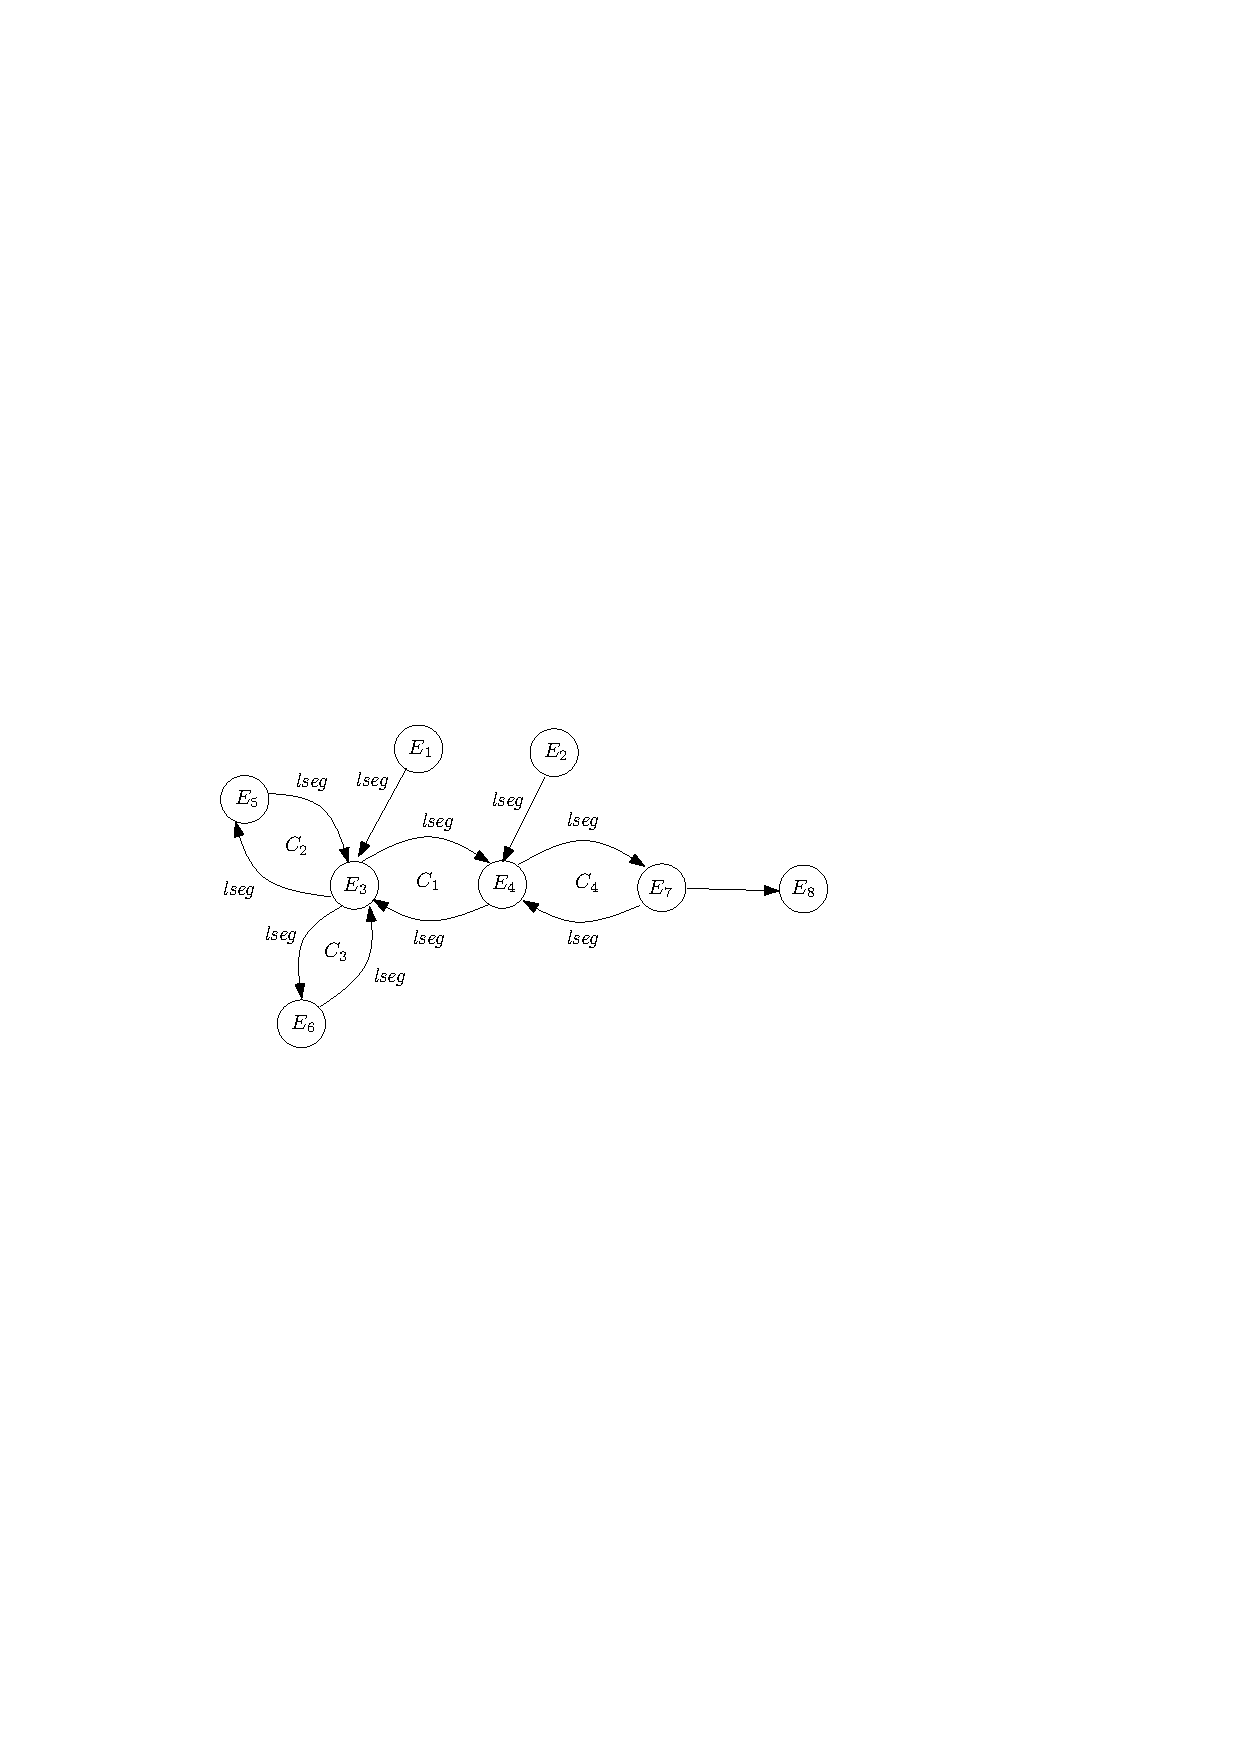
\includegraphics[scale=0.61]{scc-example.pdf}
\end{center}
\vspace{-6mm}
\caption{The structure of SCCs}
\label{fig-scc}
\vspace{-6mm}
\end{figure}

\begin{example}\label{exmp-scc}
Suppose $\varphi = \lseg(E_1; E_3) \sep \lseg(E_2; E_4) \sep \lseg(E_3; E_4) \sep \lseg(E_4; E_3) \sep \lseg(E_3; E_5) \sep \lseg(E_5; E_3) \sep \lseg(E_3; E_6) \sep \lseg(E_6;  E_3) \sep \lseg(E_4; E_7) \sep \lseg(E_7; E_4) \sep \lseg(E_7; E_8)$. Then the graph $\Gg'_\varphi$ has just one nontrivial SCC as shown in Fig.~\ref{fig-scc}.
\end{example}

%Consider any SCC $C$ and a node $v\in C$, we have the following cases:
%\begin{itemize}
%\item $v$ has only one field-labelled arc;
%
%\item $v$ is not allocated and none of nodes in $C$ are allocated;
%
%\item $v$ is allocated and there is one field-labelled arc in $C$, then $C$ must be of the form of single cycle (i.e., $C$ is deterministic; each node in $C$ has a unique successor). In this case, must $C$ be final?
%
%\item $v$ is allocated, but there is no field-labelled arc in $C$ (for instance $y\neq z \wedge ls(x,y)\sep ls(x,z)$)
%Can we say that for each tree in the SCC graph (which is a forest), there is only one leave which is allocated?
%\end{itemize}

\begin{proposition}\label{prop-sl-pred-arc}
Let $v$ be an allocated node in $\Gg'_\varphi$ such that all the arcs out of $v$ are predicate-labeled. Moreover, let $\Cc$ be the SCC to which $v$ belongs.
\begin{itemize}
\item
If $\Cc$ is non-final and non-trivial, then any node which is outside of $\Cc$ and is reachable from $\Cc$ must \emph{not} be allocated.
%
\item If there is a field-labeled arc in $\Cc$, then $\Cc$ comprises just one simple cycle and $\Ee(v)=\Cc$. (That is, $\Cc$ contains all the arcs reachable from $v$.)
\end{itemize}
\end{proposition}

Then in the rest of this subsection, let us assume that $\varphi$ and $\psi$ be two SLID[$\lseg$] formulae such that $\lvars(\psi) \subseteq \lvars(\varphi)$. Our goal is to solve the entailment problem $\varphi \models \psi$.

The idea is to reduce the entailment problem to the existence of a homomorphism from $\Gg'_\psi$ to $\Gg'_\varphi$ (in normal forms) and show that the existence of homomorphisms can be decided in polynomial time.


\hide{
\begin{proposition}
Suppose $\varphi \models \psi$ and $E,F \in \lvars(\psi)$. Let $\Cc$ be a connected component of $\Gg'_\psi$ and $\lvars(\Cc) = \bigcup \limits_{v \in \Cc} \Ll'_{\psi,1}(v)$. Then there is a connected component $\Cc'$ of $\Gg'_\varphi$ such that $\lvars(\Cc) \subseteq \lvars(\Cc')$.
\end{proposition}
\fu{From the aforementioned definition, $\Ll'_{\psi,1}([E])=[E]$.} \zhilin{Yes. But since we get the graph $\Gg'_\psi$ by merging some nodes, $\Ll'_{\psi,1}(v) \neq [E]_{\Pi_2}$ anymore if $E \in \Ll_{\psi,1}(v)$.}\fu{The update of $\Ll'_{\psi,1}$ was not mentioned when merging. }

Intuitively, the above proposition says that the set of location variables occurring in a connected component of $\Gg'_\varphi$, except those that only occurring in $\varphi$ (but not in $\psi$), is the union of those occurring in several connected components of $\Gg'_\psi$.
\fu{Sorry, it is difficult for me to see this intuition from the above proposition.} \zhilin{Yes. We need polish it.}

In the following, we first show how to decide the entailment $\varphi \vDash \psi$ by considering the special case that $\Gg'_\varphi$ is connected. Then we will extend the decision procedure to the more general case later.


Suppose that $\Gg'_\varphi = (\Vv'_\varphi, \Rr'_\varphi, \Ll'_{\varphi,1}, \Ll'_{\varphi,2})$ is connected.
}

At first, let us use the following two examples to get an idea of the homomorphism. The basic idea of the homomorphism is to match a node containing a variable in $\Gg'_\psi$ to the node containing the same variable in $\Gg'_\varphi$. Moreover, each arc in $\Gg'_\psi$ is matched to the simple path in $\Gg'_\varphi$ between the two nodes in $\Gg'_\varphi$ which are the counterparts of the two endpoints of the arc, if the two nodes are distinct from each other.

\begin{example}\label{entl-exmp-1}
Let $\varphi = \lseg(E_1; E_2) * \lseg(E_2; E_3) * \lseg(E_3; E_2) * \lseg(E_2; E_4)$ and $\psi = \lseg(E_1; E_4)$. Then the graph $\Gg'_\varphi$ and $\Gg'_\psi$ are as in Fig.~\ref{fig-entl-example-1}.  It is not hard to see that the entailment $\varphi \models \psi$ holds. The homomorphism from $\Gg'_\psi$ to $\Gg_\varphi$ matches $E_1$ to $E_1$ and $E_4$ to $E_4$. Moreover, in the homomorphism, the arc from $E_1$ to $E_4$ in $\Gg'_\psi$ is matched to the simple path from $E_1$ to $E_4$ in $\Gg'_\varphi$. No arcs from the cycle in $\Gg'_\varphi$ are covered by any simple path of $\Gg'_\varphi$ matching some arc in $\Gg'_\psi$.
\end{example}


\begin{figure}[htbp]
\begin{center}
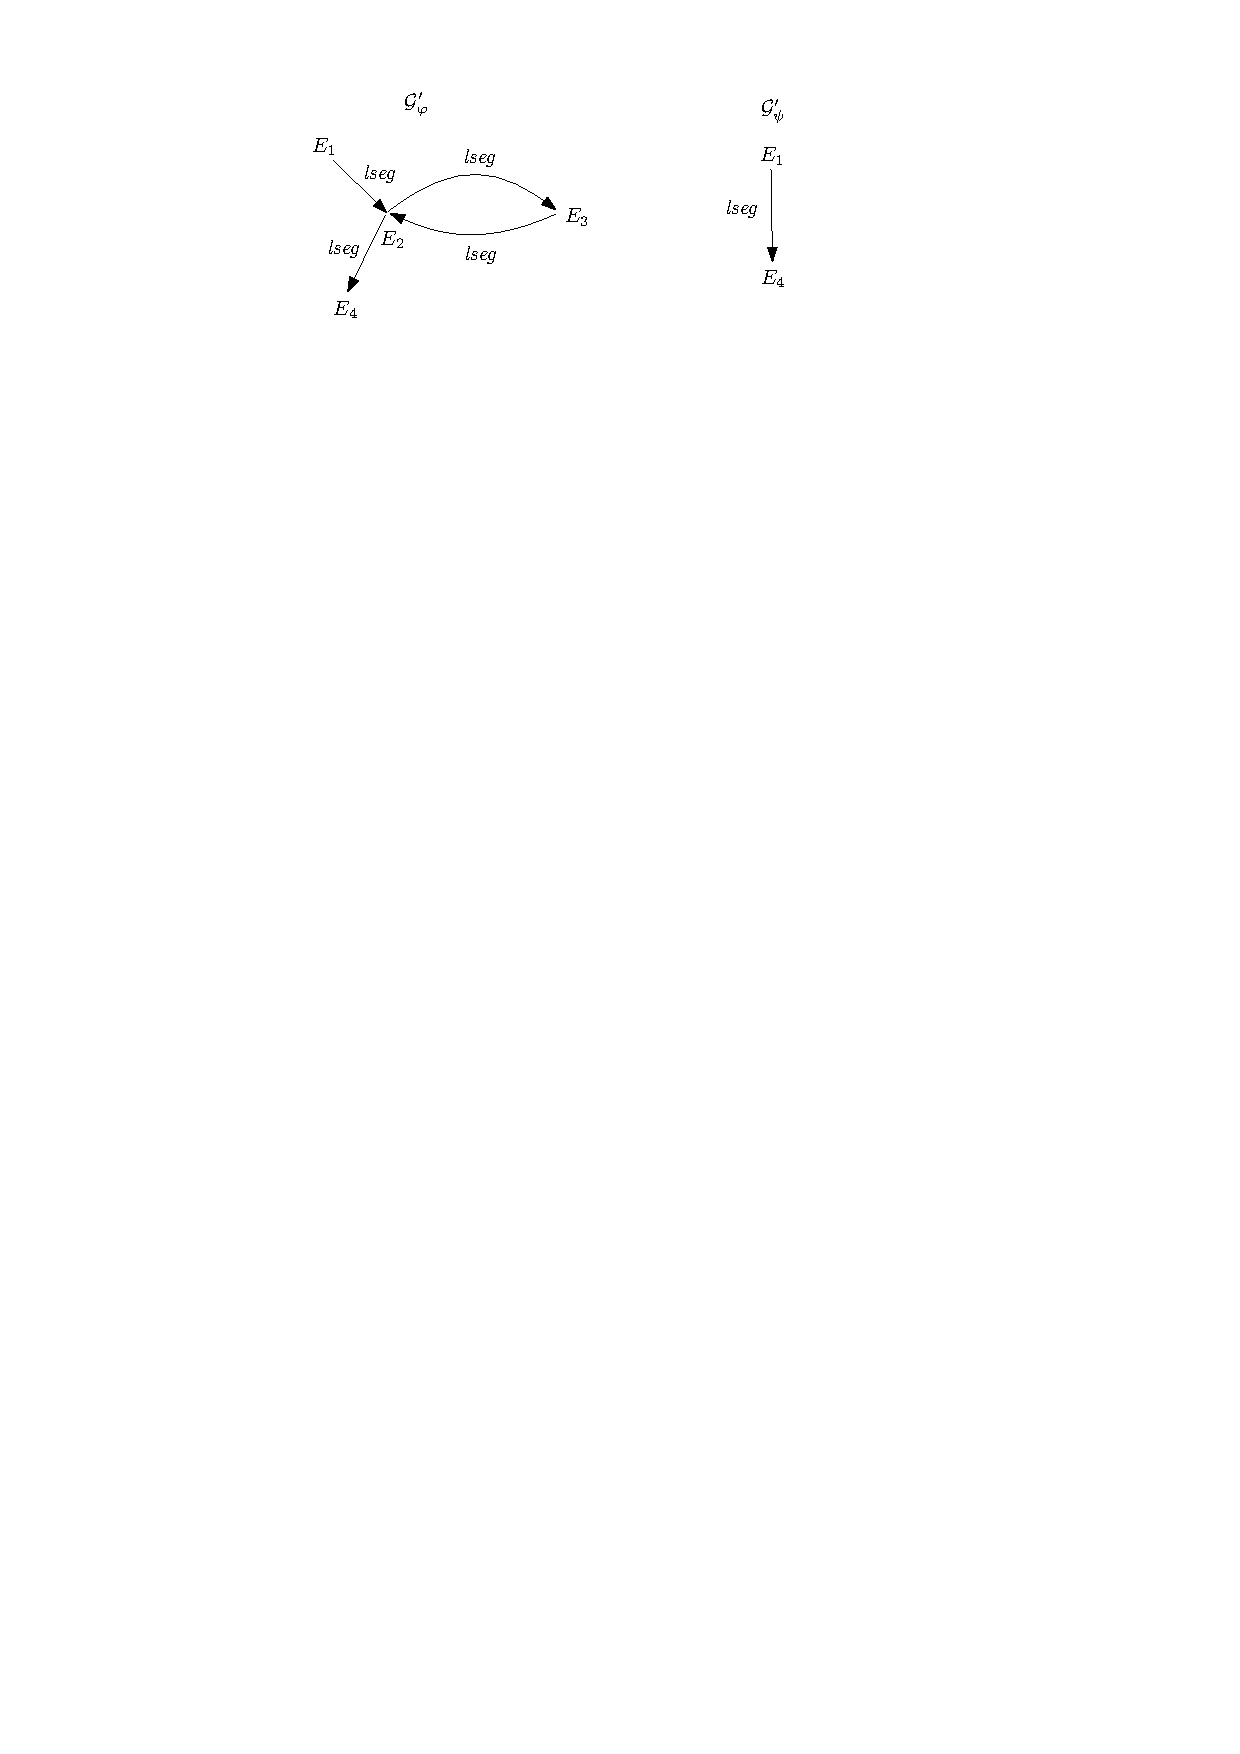
\includegraphics[scale=0.6]{entl-example-1.pdf}
\end{center}
\caption{Graph $\Gg'_\varphi$ and $\Gg'_\psi$}\label{fig-entl-example-1}
\end{figure}


\begin{example}\label{entl-exmp-2}
Let $\varphi = \lseg(E_1; E_2) * \lseg(E_2; E_3) * \lseg(E_3; E_2) * \lseg(E_3; E_4)$ and $\psi = \lseg(E_1; E_4)$. Then the graph $\Gg'_\varphi$ and $\Gg'_\psi$ are as in Fig.~\ref{fig-entl-example-2}.    It is not hard to see that the entailment $\varphi \models \psi$ does not hold. The homomorphism from $\Gg'_\psi$ to $\Gg_\varphi$ matches $E_1$ to $E_1$ and $E_4$ to $E_4$. Moreover, in the homomorphism, the arc from $E_1$ to $E_4$ in $\Gg'_\psi$ is matched to the simple path from $E_1$ to $E_4$ in $\Gg'_\varphi$, which includes an arc from $E_2$ to $E_3$ in the cycle of $\Gg'_\varphi$.  Moreover, the arc from $E_3$ to $E_2$ in the cycle is not covered by any simple path matching to some arc in $\Gg'_\psi$.
\end{example}

\begin{figure}[htbp]
\begin{center}
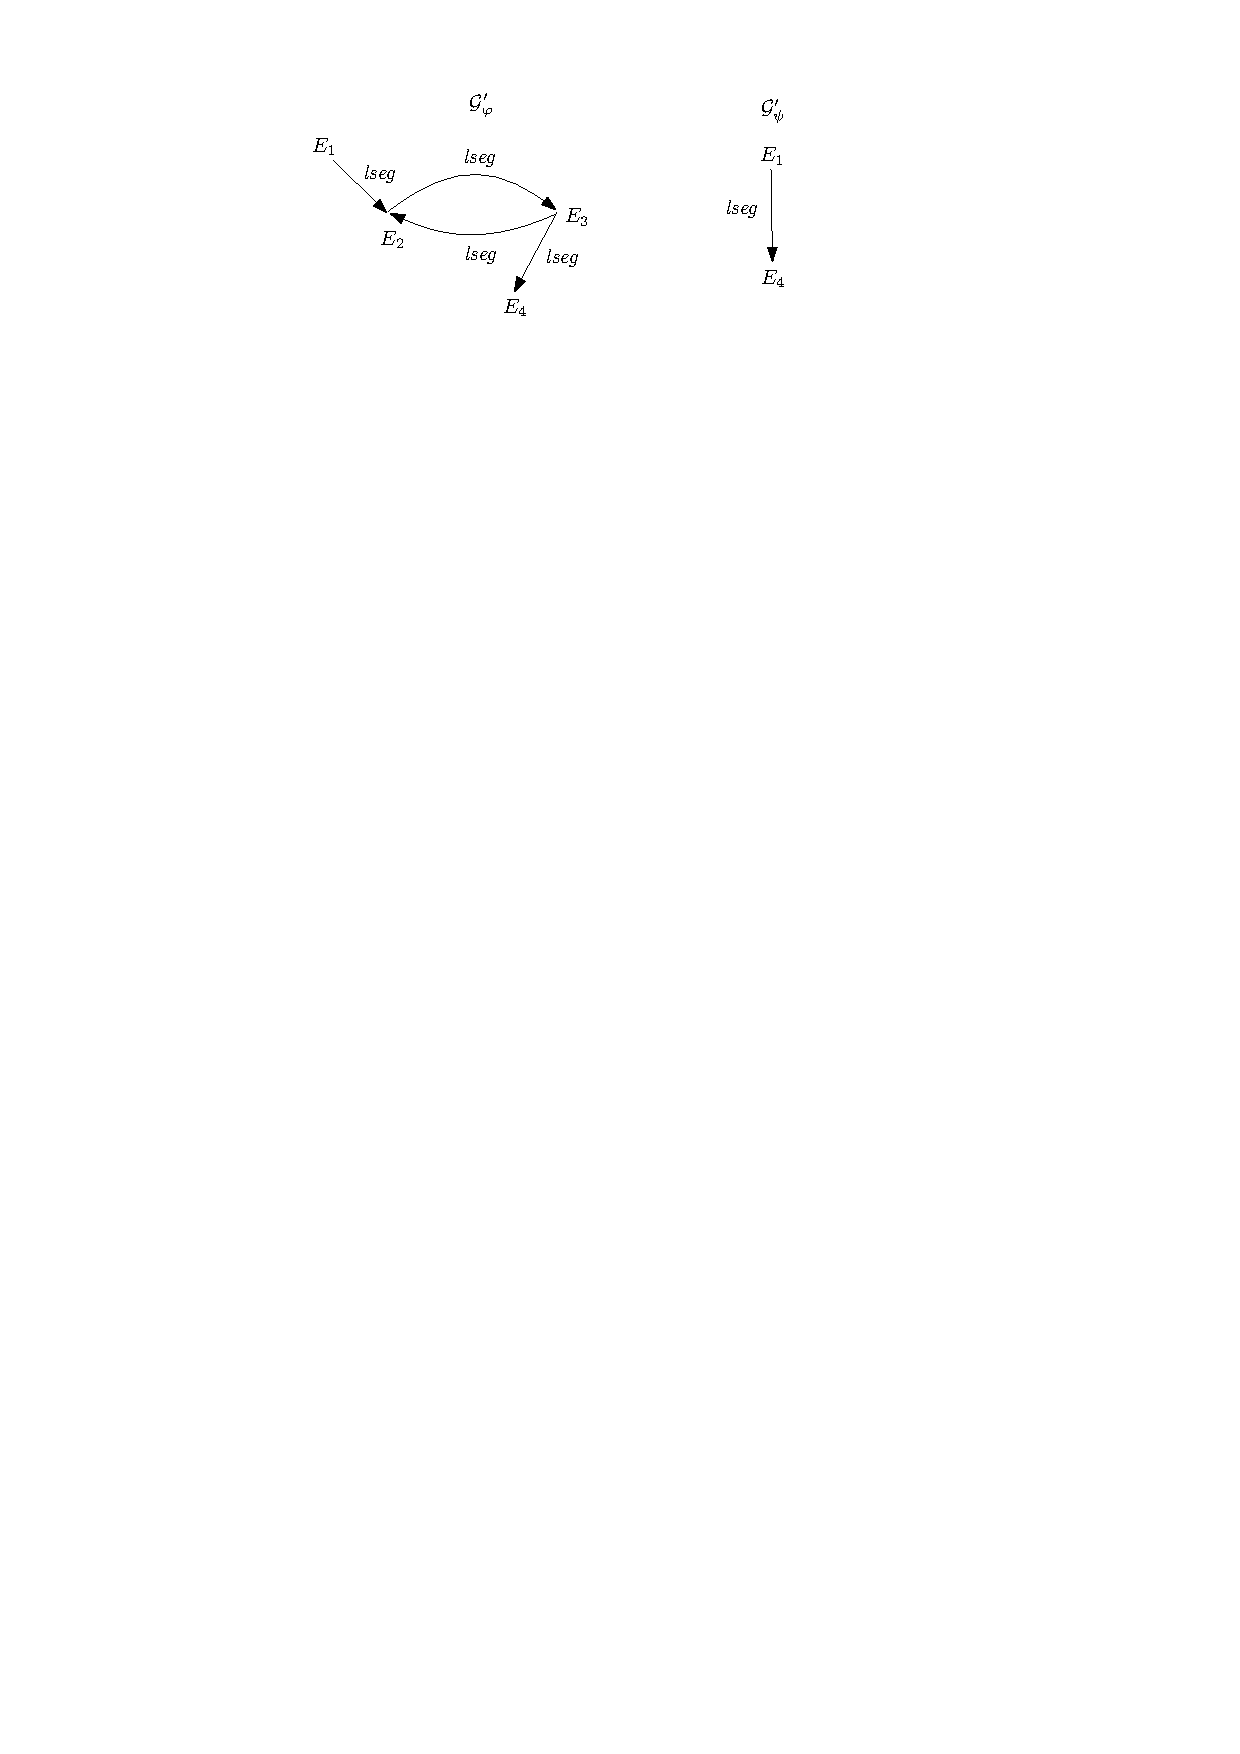
\includegraphics[scale=0.6]{entl-example-2.pdf}
\end{center}
\caption{Graph $\Gg'_\varphi$ and $\Gg'_\psi$}\label{fig-entl-example-2}
\end{figure}

The homomorphism in Example~\ref{entl-exmp-1} is different from that in Example~\ref{entl-exmp-2} as follows: In Example~\ref{entl-exmp-1}, no arcs in the cycle are covered by the simple paths matching to the arcs in $\Gg'_\psi$, whereas in Example~\ref{entl-exmp-2}, the arcs in the cycle are \emph{partially} covered.

\begin{definition}[{Homomorphism from $\Gg'_\psi$ to $\Gg'_\varphi$}]\label{def-hom-sleg}
A homomorphism from $\Gg_\psi$  to $\Gg_\varphi$ is a function $\theta: \Vv'_\psi \rightarrow \Vv'_{\varphi}$ such that
\begin{itemize}
\item{\bf variable subsumption}: for each $v \in \Vv'_{\psi}$, $\Ll'_{\psi,1}(v) \subseteq \Ll'_{\varphi,1}(\theta(v))$,
%
%\item{\bf $\theta$ is uniquely determined}: for each $E \in \lvars(\psi)$ and each node $v \in \Vv'_{\psi}$ such that $E \in \Ll'_{\psi,1}(v)$, it holds that $\theta(v)=v'$ such that $E \in \Ll'_{C,\varphi,1}(v')$,
%
\item{\bf field-labeled arcs}: for each field-labeled arc $e$ from $v$ to $w$ in $\Gg'_{\psi}$, there is a  field-labeled arc from $\theta(v)$ to $\theta(w)$ in $\Gg'_{\varphi}$ --- this arc in $\Gg'_{\varphi}$ is said to be assigned to $e$, denoted by $\eta(e)$,
%
\item{\bf predicate-labeled arcs}: for each predicate-labeled arc $e$ from $v$ to $w$ in $\Gg'_{\psi}$, if $\theta(v) \neq \theta(w)$, then there is a (unique) simple path from $\theta(v)$ to $\theta(w)$ in $\Gg'_{\varphi}$ --- this simple path is said to be assigned to $e$, denoted by $\eta(e)$,
%
\item {\bf undirected arcs}: for each undirected arc between $v$ and $w$ in $\Gg'_\psi$, there is an undirected arc between $\theta(v)$ and $\theta(w)$,

\item {\bf separation constraint}: for each pair of distinct arcs $e_1,e_2$ in $\Gg'_\psi$ such that $\eta(e_1),\eta(e_2)$ are defined, it holds that $\eta(e_1)$ and $\eta(e_2)$ are arc-disjoint,
%
%\item {\bf initial and final SCCs}: each initial SCC $v'$ in $\Gg'_{C,\varphi}$ is in  $\rng(\theta)$, moreover, $C$, as the unique final SCC, contains at least one node from $\rng(\theta)$,
%
\item {\bf coverage of all the arcs in $\Gg'_{\varphi}$, except the nontrivial SCCs}: each arc of $\Gg_{\varphi}$ that does not belong to any nontrivial SCC occurs in $\eta(e)$ for some arc $e$ in $\Gg'_{\psi}$, moreover, the nontrivial SCCs of $\Gg'_\varphi$ satisfy the following two constraints,
\begin{itemize}
\item for each nontrivial SCC $\Cc$ of $\Gg'_\varphi$ which is a CC at the same time, each arc of $\Cc$ occurs in $\eta(e)$ for some arc $e$ in $\Gg'_\psi$,
%
\item for each nontrivial SCC $\Cc$ of $\Gg'_\varphi$ which is not a CC, either each arc of $\Cc$ occurs in $\eta(e)$ for some arc $e$ in $\Gg'_{\psi}$, or none of the arcs of $\Cc$ satisfies this property.
\end{itemize}
    \fu{The later condition on nontrivial SCC as well as the augment on the difference of two examples are difficult to understand.  }
\end{itemize}
\end{definition}

%\begin{lemma}
%For any graph in normal form, if $v$ is allocated,
%\end{lemma}

\begin{lemma}
$\varphi  \models \psi$ iff there is a homomorphism from $\Gg_\psi$ to $\Gg_\varphi$.
\end{lemma}

%\tl{is this a counterexample?
%$\varphi= ls(x,y)\sep ls(y,z) \sep ls(z,y)$ and $\psi = ls(x,y)$
%}

\zhilin{
I briefly describe my idea of the proof.

``only if'' direction: Suppose there does not exist a homomorphism from $\Gg_\psi$ to $\Gg_\varphi$, we show that $\varphi \not \models \psi$.

then the function $\theta: \Vv_\psi \rightarrow \Vv_\varphi$ violates at least one of the six constraints in the def of homomorphisms. then from these violations, we show that there exists a state $(s,h)$ such that $(s,h) \models \varphi$, but $(s,h) \not \models \psi$.



``if'' direction: suppose there is a homomorphism from $\Gg_\psi$ to $\Gg_\varphi$ and $(s,h) \models \varphi$, we want to show that $(s,h) \models \psi$.

For each arc $e$ from $[E]_\psi$ to $[F]_\psi$ in $\Gg_\psi$, we define a subheap of $h_e$ of $h$ as follows.
\begin{itemize}
\item If $e$ is field-labeled, then $h_e$ is the subheap of $h$ corresponding to $\eta(e)$.
%
\item If $e$ is predicate-labeled and $[E]_\varphi \neq [F]_\varphi$, then for each nontrivial SCC $\Cc$ of $\Gg_\varphi$ that is reachable from $[E]_\varphi$ and co-reachable from $[F]_\varphi$ such that none of the arcs of $\Cc$ occurs in $\eta(e')$ for some $e'$ in $\Gg_\psi$, then let $h_e$ be the subheap of $h$ corresponding to the union of $\eta(e)$ and all such SCCs that are reachable from $[E]_\varphi$ and co-reachable from $[F]_\varphi$.
\end{itemize}

Then we can show that $(s,h_e) \models \Sigma_e$, where $\Sigma_e$ is the predicate atom corresponding to $e$. From this, we conclude $(s,h) \models \psi$.
}




\begin{proof} Suppose $\varphi=\Pi \wedge \Sigma$
and $\psi=\Pi'\wedge \Sigma'$, where $\Sigma\equiv a_1 \sep \dots \sep a_n$ and $\Sigma'\equiv a_1' \sep \dots \sep a'_{n'}$. We consider two directions.
% there is an example which is interesting for the proof:
% E1 -> F1-> E2, E3->F2-> E4, and F1 and F2 form a loop.

Suppose that there is a homomorphism $\theta$ from $\Gg_\psi$ to $\Gg_\varphi$, and there is a model $(s, h)\models \Gg_\varphi$. For each edge $e$ in $\Gg_\psi$, according to Definition~\ref{def-hom-sleg}, we have a corresponding path $\eta(e)$ in $\Gg_\varphi$ for which we have a corresponding subheap $h(e)$. Clearly $(s, h(e))\models e$ \fu{$(s, h(e))\models a'_{i(e)}$}.  By the separation constraint, we have that \fu{ for every $e,e'$ in $\Gg_\psi$, if $e\neq e'$ then $h(e)\sharp h(e')$}, i.e., they are domain disjoint.

Let $\hbar:=h\setminus \sep_{e\in \Gg_\psi} h(e)$ \fu{$\hbar:=h\setminus \biguplus_{e\in \Gg_\psi} h(e)$?}. If $\dom(\hbar)=\emptyset$, then cleary $h= \sep_{e\in \Gg_\psi} h(e)\models \Gg_\psi$ \fu{$(s,\biguplus_{e\in \Gg_\psi} h(e))\models \psi$?? }, and we are done. Otherwise, by the coverage constraint, it must be the case that $\hbar$ contains a set of non-trivial SCCs of $\Gg_\varphi$,  the edges of each of which are all included in $\hbar$. Fix one such SCC $C$, and write $\hbar_C$ to be the subheap of $\hbar$ corresponding to $C$. As $\hbar$ is a function (thus ``deterministic"), it must be the case that $\hbar_C$ is of the form $h(l_i, \mathsf{next})=l_{i+1}$ for $i\geq 1$ and $l_{n+1}= l_1$.

As the SCC $C$ is not isolated, there exists a node $v\in \Gg_\varphi$ such that $v$ appears in the path $\eta(e)$ for some $e\in \Gg_\psi$ and $s(x)=l_1$ where $x$ is a variable in $v$. Moreover, $l_1\notin \dom(h(e))$. It is then not difficult to see that  $\hbar_C\uplus h(e)\models e$ \fu{$(s,\hbar_C\uplus h(e))\models a_{i(e)}$?}.  We then define $\tilde{h}(e):= \hbar_C\uplus h(e)$. It follows that
$h= \sep_{e\in \Gg_\psi} \tilde{h}(e)\models \Gg_\psi$ \fu{$(s,\biguplus_{e\in \Gg_\psi} \tilde{h}(e))\models \psi$??}.

%To conclude, we can distribute $\hbar$ (if not empty) to


%some $l$ such that
%$l$ appears in some $\eta(e)$ and $l=l_1$.

%We now consider a partition of the set of edges of $\Gg_\varphi$ according to $\Gg_\psi$ and $(s, h)$. For each edge $e\in \Gg_\psi$,
%
%\begin{itemize}
%\item if $e$ is field-labeled. Then according to Definition~\ref{def-hom}, %we must have an edge $(\theta(u), \theta(v))$ in $\Gg_\varphi$;
%the corresponding part is $\eta(e)$;
%
%\item if $e$ is predicate-labeled. Then the corresponding part is $\eta$ together with all non-trivial SCCs which are not assigned at all and connect to $\eta(e)$.
%
%\end{itemize}
%
%To see why this is a partition. by connecting to $\eta(e)$, we mean one of the nodes along the path $\eta(e)$ belongs to the SCC.
%Then for each edge in $\Gg_\varphi$, we have a corresponding subheap satisfying the edge.

%====================
%For each edge $e=(u, v)$ of $\Gg_\psi$, we consider the following cases:
%\begin{itemize}
%\item $e$ is field labeled. Then according to Definition~\ref{def-hom}, we must have an edge $(\theta(u), \theta(v))$ in $\Gg_\varphi$ which is also field labeled. Clearly, $h(s(\theta(u)), \mathsf{next})= s(\theta(v))$.
%
%\item $e$ is predicate labeled. Then we have a unique simple path $\eta(e)$ from $\theta(u)$ to $\theta(v)$ in $\Gg_\varphi$. %We have a case distinction here:
%%\begin{itemize}
%%\item $s(\theta(u))\neq s(\theta(v))$. Consider the subheap of $h$ corresponding to this simple path $\eta(e)$,  it is not difficult to see that this subheap satisfies $e$.
%%\item $s(\theta(u))=s(\theta(v))$.
%%Then
%By the separation constraint,  $\eta(e)$ must consist of predicate-labeled arcs only.
%% for each node $w$ along this path,  $l:=s(\theta(u))=s(\theta(v))=s(w)$.
%%If $l\not\in \dom(h)$, we are done. Otherwise,
%Clearly, $s(\theta(u)), s(\theta(v))\in \dom(h)$ (which might be equivalent). Consider the subheap $h'$ of $h$ which starts from $s(\theta(u))=l_0$, and is given by  $h(l_i, \mathsf{next})=l_{i+1}$ for $i\geq 1$ and $l_n= s(\theta(v))$. Clearly as $h'$ is deterministic, we have that if $h'$ contains one non-trivial SCC, $h'$ contains exactly one non-trivial SCC.
%
%%there must be a subheap of $h$, corresponding to a cycle of in $\Gg_\varphi$, such that $h(l, \mathsf{next})=l_1$, $h(l_1, \mathsf{next})=l_2$, ..., $h(l_n, \mathsf{next})=l$. This subheap satisfies $e$ as well.
%\end{itemize}
%
%
%\tl{it is only a sketch here, in the proof, you need to consider merge of nodes, etc}
%In summary, for each edge $e$ in $\Gg_\psi$, we have find a subheap $h(e)$ of $h$ such that $h(e)\models e$. By the separation constraint, we have that for $e\neq e'$, $h(e)\sharp h(e')$, i.e., they are domain disjoint. Hence we have that $\sep_{e\in \Gg_\varphi} h(e)\models \Gg_\varphi$.
%
%We then have to argue that $h$ has nothing left.  To this aim, we consider $\hbar:=h\setminus \sep_{e\in \Gg_\varphi} h(e)$. By the last condition of Definition~\ref{def-hom}, $\hbar$ must correspond to a set of nontrivial SCCs because otherwise it would have been ``covered" already.
%
%Note that $h$, as a model of $\Gg_\varphi$, has to cover each edge of $\Gg_\varphi$.
%Suppose $\hbar$ is a link $l_1\mapsto l_2\cdots \mapsto l_n$. Clearly, the nodes which are mapped by $s$ to $l_1$ and $l_n$ must be considered before.
%
%
%The only possibility is that $l_1=l_n$. Then it must be the case that the cycle is "final". However, this has been covered before.


 %Moreover, each node in these SCCs must not appear in the domain of $\sep_{e\in \Gg_\varphi} h(e)$.

 \medskip

For the other direction, assuming $\varphi\models \psi$, obvious a mapping $\theta$ respecting the variable subsumption can be defined, as otherwise $\varphi\not\models \psi$ trivially. We then show that $\theta$ must satisfy the remaining constraints by contradiction.

\begin{itemize}
\item field-labeled arcs: trivial;
\item undirected arcs: trivial;
\item separation constraint: trivial.
\item predicate-labeled arcs: if there is no path from $\theta(u)$ to $\theta(v)$, then any model of $\varphi$ cannot contain a list from $s(\theta(u))$ to $s(\theta(v))$. Any such a model does not satisfy $\psi$.

\item coverage:  we shall consider the following possible violations:
\begin{itemize}
\item there is an arc  $(u,v)\in \Gg_\varphi$ which does not belong to any nontrivial SCC, but does not appear in any $\eta(e)$ for $e\in \Gg_\psi$.  Then we can construct a model $(s,h)$ such that $s(u)\neq s(v)$ and $h(s(u))=s(v)$. Clearly $(s,h)\not\models \psi$ because of the classical \fu(non-intuitionistic) semantics.

\item
\end{itemize}
\end{itemize}





\end{proof}

\begin{theorem}
The entailment of two SLID[$\lseg$] formulae can be decided in polynomial time.
\end{theorem}



\hide{


%\begin{lemma}
%We can construct an SL-graph $G$ in normal form for a given formula $\Pi\wedge \Sigma$ in polynomial time.
%\end{lemma}
%
%\begin{definition}
%Let $G, G'$ be two SL-graphs in normal form. A mapping $h: V_{b,r}\rightarrow V_{b,r}'$ is a homomorphism from $G$ to $G'$ if
%\begin{itemize}
%\item $vars(h(v))\supseteq vars(v)$;
%\item $h$ preserves $E_d$;
%\item $h$ preserves $E_{p,swarrow}$ and $E_{p, searrow}$;
%\item similar to the previous case;
%\item
%\end{itemize}
%\end{definition}

%\begin{definition}[Allocated nodes] A node $v$ is \emph{allocated} if
%\begin{itemize}
%\item there is a field-labled arc from $v$;
%\item $v\rightarrow_l w_1$ and $v\rightarrow_l w_2$ and $\{w_1, w_2\}\in E_d$.
%
%\item if $v\rightarrow_l w$ and $w$ is allocated
%
%\item if $v\rightarrow_l w$ and $(v, w)\in E_d$.
%\end{itemize}
%\end{definition}

The problem of dll lies in that even if the graph is reduced, still it is not trivial to decide whether a model exists. For instance
$dll(E, P; F, L)\sep dll(L, -; F', L')$. One of them (or both) must be emp.

To this end, it might be help to consider the extended $\rightarrow_l$ relation, namely, $dll(E, P; F, L)$ gives $E\stackrel{L}{\rightarrow}_l F$, and for the reduced graph, we have that: if $E\stackrel{L}{\rightarrow}_l F$ and $L$ is allocated, then $E=F$ and $P=L$.

Then the question is if we have two arcs in $E_l$ such that $E\stackrel{L}{\rightarrow}_l F$ and $L\stackrel{L'}{\rightarrow}_l F'$, is the graph reduced? This depends ...
}

\subsection{SLID[$\thole$]}

The challenge here is to give a proper definition of the matching of a subgraph to a predicate-labeled arc.

\begin{definition}
Given two nodes of $\Gg_\varphi$, $u, v$, we define  a predicate $u\leadsto v$ inductively:
\begin{itemize}
\item $u=v$;
\item $u\mapsto [(\mathsf{left}, w_1), (\mathsf{right}, w_2) ]$ and either $w_1\leadsto v$ or $w_2\leadsto v$;
\item there is an edge $(u,w)$ labeled by dllseg, and $w\leadsto v$.
\end{itemize}

Suppose $u\leadsto v$, we define the subgraph $\mathcal{T}(u,v)$.
\end{definition}
\zhilin{I am not sure the definition of $u \leadsto v$ is correct. I think the second item above should be: $u \mapsto [(\mathsf{left}, w_1), (\mathsf{right}, w_2) ]$, moreover, either $w_1 \leadsto v$ and $w_2 \leadsto \nil$, or $w_1 \leadsto \nil$ and $w_2 \leadsto v$.}

\begin{definition}[{Homomorphism from $\Gg_\psi$ to $\Gg_\varphi$}]\label{def-hom}
A homomorphism from $\Gg_\psi$  to $\Gg_\varphi$ is a function $\theta: \Vv_\psi \rightarrow \Vv_{\varphi}$ such that
\begin{itemize}
\item{\bf variable subsumption}: for each $v \in \Vv'_{\psi}$, $\Ll'_{\psi,1}(v) \subseteq \Ll'_{\varphi,1}(\theta(v))$,
%
%\item{\bf $\theta$ is uniquely determined}: for each $E \in \lvars(\psi)$ and each node $v \in \Vv'_{\psi}$ such that $E \in \Ll'_{\psi,1}(v)$, it holds that $\theta(v)=v'$ such that $E \in \Ll'_{C,\varphi,1}(v')$,
%
\item{\bf field-labeled arcs}: for each field-labeled arc $e$ from $v$ to $(w_l, w_r)$ in $\Gg_{\psi}$, there is a  field-labeled arc from $\theta(v)$ to $(\theta(w_l), \theta(w_r))$ in $\Gg_{\varphi}$ --- this arc in $\Gg_{\varphi}$ is said to be assigned to $e$, denoted by $\eta(e)$,
%
\item{\bf predicate-labeled arcs}: for each predicate-labeled arc $e$ from $v$ to $w$ in $\Gg_{\psi}$, if $\theta(v) \neq \theta(w)$, then $\theta(u)\leadsto \theta(v)$ %there is a (unique) simple path from $\theta(v)$ to $\theta(w)$
in $\Gg_{\varphi}$ --- the tree $\mathcal{T}(\theta(u), \theta(v))$ is said to be assigned to $e$, denoted by $\eta(e)$ \fu{$\theta(v)$ should be $\theta(w)$?},
%
\item {\bf undirected arcs}: for each undirected arc between $v$ and $w$ in $\Gg_\psi$, there is an undirected arc between $\theta(v)$ and $\theta(w)$,

\item {\bf separation constraint}: for each pair of distinct arcs $e_1,e_2$ in $\Gg_\psi$ such that $\eta(e_1),\eta(e_2)$ are defined, it holds that $\eta(e_1)$ and $\eta(e_2)$ are arc-disjoint,
%
%\item {\bf initial and final SCCs}: each initial SCC $v'$ in $\Gg'_{C,\varphi}$ is in  $\rng(\theta)$, moreover, $C$, as the unique final SCC, contains at least one node from $\rng(\theta)$,
%
\item {\bf coverage of all the arcs in $\Gg_{\varphi}$, except the nontrivial SCCs}: each arc of $\Gg_{\varphi}$ that does not belong to any nontrivial SCC occurs in $\eta(e)$ for some arc $e$ in $\Gg_{\psi}$, moreover, the nontrivial SCCs of $\Gg_\varphi$ satisfy the following two constraints,
\begin{itemize}
\item for each nontrivial SCC $\Cc$ of $\Gg_\varphi$ which is a CC at the same time, each arc of $\Cc$ occurs in $\eta(e)$ for some arc $e$ in $\Gg_\psi$,
%
\item for each nontrivial SCC $\Cc$ of $\Gg_\varphi$ which is not a CC, either each arc of $\Cc$ occurs in $\eta(e)$ for some arc $e$ in $\Gg_{\psi}$, or none of the arcs of $\Cc$ satisfies this property.
\end{itemize}

\end{itemize}
\end{definition}

\subsection{SLID[$\dllseg$]}




\tl{
The problem here is that, suppose we have obtained a graph in normal form (as in the previous case, and all good properties are preserved), we might have the case $dll(E, P; F, L)\sep dll(L, -; F', L')$ where $E$ to $F$ has an edge and $L$ has an edge to $F'$. Different from the lseg case, here these two edges are not connected in graph, but in any model, one of them must be an empty subheap. I have not thought carefully, but when one defines the homomorphism, MAYBE some edges do not need to be covered,
}


\zhilin{In the following, I try to sketch the decision procedure for entailment problem of $\dllseg$. The decision procedure simplifies $\Gg_\varphi$ into a collection of graphs and consider homomorphisms from $\Gg_\psi$ to each o them.}

With the concept of allocated nodes, we can also obtain a normal form $\Gg'_\varphi$ from $\Gg_\varphi$, where $\varphi$ is a SLID$[\dllseg]$ formula.


We first assume that $\Gg'_\varphi$ is connected, then we show how to extend the arguments to the more general case.

The decision procedure proceeds as follows: For each simple cycle $C$ in $\Gg'_\varphi$, we obtain a graph $\ctr_C[\Gg'_\varphi]$ from $\Gg'_\varphi$ by contracting all  nodes in $\Gg'_\varphi$ that are reachable from, but are outside of, $C$. Moreover, we consider another graph $\ctr_{scc}[\Gg'_\varphi]$ obtained from $\Gg'_\varphi$ by contracting all  nontrivial SCCs in $\Gg'_\varphi$ (cf. Definition~\ref{def-ctr}). The entailment problem is then reduced to a series of checking whether a homomorphism exists for a pair of graphs, i.e.,  %as follows: $\varphi \models \psi$ iff
whether there exist homomorphisms from $ \Gg'_\psi$ to $\ctr_{scc}[\Gg'_\varphi]$ and %whether there is a homomorphism from $(\boolabs(\psi), \Gg_\psi)$
to $\ctr_C[\Gg'_\varphi]$ for each simple cycle $C$ in $\Gg'_\varphi$; cf. Definition~\ref{def-hom-scc}-\ref{def-hom-cycle}.

To define these contractions properly, we first introduce some additional notations.
Let $C$ be a simple cycle in $\Gg'_\varphi$. For each node $[F]$ reachable from $C$ and outside of $C$, we see a node $[E]$ in $C$ \emph{owns} $[F]$ if each path starting from some node in $C$ and ending in $[F]$ must go through $[E]$. From Proposition~\ref{prop-cycle}, we know that for each node $[F]$ reachable from $C$ and outside of $C$, there is a unique node $[E]$ in $C$ which owns $[F]$. Moreover, for each arc $e$ reachable from $C$ and not belonging to $C$, $e$ is said to be owned by a node $[E]$ in $C$ if either the source node or the destination node of $e$ is owned by $[E]$. We call a node $[E]$ in $C$ that owns at least one node as an \emph{out-port} node.

%For instance, consider the simple cycle $C_1$ of $\Gg'_\varphi$ in Fig.~\ref{fig-scc}, we know that $[E_4]$ owns $[E_6]$, $[E_3]$ owns $[E_5]$, moreover, $[E_3]$ owns the arc from $[E_3]$ to $[E_5]$ as well as the arc from $[E_5]$ to $[E_3]$, and the out-port nodes of $C$ are $[E_3]$ and $[E_4]$.

\begin{definition}[{$C$-contraction and SCC-contraction}]\label{def-ctr}
Let $C$ be a simple cycle in $\Gg'_\varphi$. Then the $C$-contraction of $(\boolabs(\varphi), \Gg'_\varphi)$, denoted $(\boolabs_C(\varphi), \ctr_{C}[\Gg'_\varphi])$, is the pair obtained from $(\boolabs(\varphi), \Gg'_\varphi)$ by applying the following three transformation steps.
%We use $[E]'$ to denote the new nodes (subsets of location variables) and
%
In the following, for a subset of nodes $\Vv'$ such that the subgraph $\Hh$ induced by $\Vv'$ is connected, we use the notation ``merge $\Hh$ into one node'' to mean that all the arcs in $\Hh$ are removed, a new node $node_{\Vv'} = \bigcup \limits_{[E] \in \Hh} [E]$ is created, and all the arcs from some node outside $\Vv'$ to some node in $\Vv'$ (resp. from some node in $\Vv'$ to some node outside $\Vv'$) are redirected to $node_{\Vv'}$ (reoriented from $node_{\Vv'}$). In addition, we use the notation ``merge two nodes $[E]$ and $[F]$'' to mean that a new node $[E] \cup [F]$ is created and all the arcs towards $[E]$ and $[F]$ (resp. from $[E]$ and $[F]$) are redirected to $[E] \cup [F]$ (resp. reoriented from $[E] \cup [F]$)
\begin{enumerate}
\item For each out-port node $[E]$ in $C$, merge the subgraph $\Hh$ induced by the union of $[E]$ and the set of nodes owned by $[E]$, into one node, moreover, for each arc $e \in \Hh$ labeled by $\dllseg(P; L)$, merge the two nodes $[P]$ and $[L]$.

\item For each nontrivial SCC $\Ss$ whose nodes are the strict ancestors of the SCC containing $C$, merge $\Ss$ into one node, and for each arc $e \in \Ss$ labeled by $\dllseg(P; L)$, merge the two nodes $[P]$ and $[L]$.

\item For each strict ancestor $[E]$ of the SCC containing $C$, merge the subgraph $\Hh$ induced by the union of $[E]$ and the set of descendants of $[E]$ that are incomparable with (the nodes in) $C$, into one node, for each arc $e \in \Hh$ labeled by $\dllseg(P; L)$, merge the two nodes $[P]$ and $[L]$.
\end{enumerate}

Moreover, we use $ \ctr_{scc}[\Gg_\varphi]$ to denote the graph obtained from $ \Gg_\varphi$ by merging $\Ss$ into one node, for each nontrivial SCC $\Ss$.
\end{definition}

Note that for each simple cycle $C$, all the nodes, except those belonging to $C$, are the ancestors of $C$ in $\ctr_C[\Gg'_\varphi]$. Moreover, $\ctr_C[\Gg'_\varphi]$ contains exactly one cycle, i.e., $C$. On the other hand, $\ctr_{scc}[\Gg'_\varphi]$ is a DAG (directed acyclic graph).

\begin{example}
Then $\ctr_C[\Gg'_\varphi]$ and $\ctr_{scc}[\Gg'_\varphi]$.
\end{example}

We use $\varphi_C$ to denote the formula corresponding to $\ctr_C[\Gg'_\varphi]$. Similarly, we use $\varphi_{scc}$ to denote the formula corresponding to $\ctr_{scc}[\Gg'_\varphi]$.


%\tl{is lemma \ref{lem-entl-red} necessary? why not just present the homo?} \zhilin{It seems for me to present the hom after the statement in the lemma is more accessible.}

\vspace{-2mm}
\begin{lemma}\label{lem-entl-red}
Let $\varphi, \psi$ be two $\lcslid[\Pp]$ formulae such that $\vars(\psi) \subseteq \vars(\varphi)$. Then $\varphi  \models \psi$ iff $\varphi_{scc} \models \psi$ and for each simple cycle $C$ of $\Gg'_\varphi$, $\varphi_C \models \psi$.
\end{lemma}
\vspace{-2mm}



From Lemma~\ref{lem-entl-red}, we know that $\varphi \models \psi$ can be reduced to a series of entailment problems $\varphi_C \models \psi$ and $\varphi_{scc} \models \psi$. In the following, we show that these problems can be further reduced to the existence of homomorphisms from $\Gg'_\psi$ to $\ctr_C[\Gg'_\varphi]$ (resp. $\ctr_{scc}[\Gg'_\varphi]$).

\begin{definition}
A path in $\Gg'_\varphi$ is matchable to an arc in $\Gg'_\psi$. \zhilin{to be done}
\end{definition}


%We start with the simpler definition of a homomorphism from $\Gg_\psi$ to $\ctr_{scc}[\Gg_\varphi]$.

\vspace{-1mm}
\begin{definition}[{Homomorphism from $\Gg'_\psi$ to $\ctr_{scc}[\Gg'_\varphi]$}]\label{def-hom-scc}
Suppose $\ctr_{scc}[\Gg'_\varphi]=$ $ (\Vv_{scc,\varphi}, \Rr_{scc,\varphi}, \Ll_{scc,\varphi})$. Then a homomorphism from $\Gg'_\psi$  to $\ctr_{scc}[\Gg'_\varphi]$ is a pair of functions $(\theta,\eta)$ such that $\theta$ is from $\Vv_\psi$ to $\Vv_{scc,\varphi}$ and $\eta$ is  from $\Ee_\psi$ to the set of simple paths in $\ctr_{scc}[\Gg'_\varphi]$ satisfying that
\begin{itemize}
\item{\bf variable subsumption}: for each node $[E] \in \Vv_{\psi}$, it holds $[E] \subseteq \theta([E])$,
%
\item{\bf field-labeled arcs}: for each field-labeled arc $e$ from $[E]$ to $[F]$ in $\Gg'_{\psi}$, $\eta(e)$ is a field-labeled arc from $\theta([E])$ to $\theta([F])$ in $\ctr_{scc}[\Gg'_{\varphi}]$,
%
\item{\bf predicate-labeled arcs}: for each predicate-labeled arc $e$ from $[E]$ to $[F]$ in $\Gg'_{\psi}$, if $\theta([E]) \neq \theta([F])$, then $\eta(e)$ is the unique simple path from $\theta([E])$ to $\theta([F])$ in $\ctr_{scc}[\Gg'_\varphi]$, otherwise, $\eta(e)$ is the empty path from $\theta([E])$ to $\theta([F])$,
%
%
\item {\bf matching of paths to arcs}: for each arc $e$ in $\Gg'_\psi$, $\eta(e)$ is matchable to $e$,

\item {\bf separation constraint}: for each pair of distinct arcs $e_1,e_2$ in $\Gg'_\psi$, it holds that $\eta(e_1)$ and $\eta(e_2)$ are arc-disjoint,
%
\item {\bf coverage of all the arcs in $\ctr_{scc}[\Gg'_{\varphi}]$}: each arc of $\ctr_{scc}[\Gg'_{\varphi}]$ occurs in $\eta(e)$ for some arc $e$ in $\Gg'_{\psi}$.
\end{itemize}
\end{definition}
\vspace{-2mm}


The definition of a homomorphism from $\Gg'_\psi$ to $\ctr_C[\Gg'_\varphi]$ turns out a bit more involved. The function $\eta(e)$ maps an arc of $\Gg'_\psi$ to either an empty path, or a simple path, or the composition of a simple path $\pi$ and the cycle $C$ such that the last node in $\pi$ belongs to $C$, moreover, $\pi$ and $C$ are arc-disjoint. We call the paths of this form as \emph{matching paths} of $\ctr_C[\Gg'_\varphi]$.

 \vspace{-2mm}
\begin{definition}[{Homomorphism from $\Gg'_\psi$  to $\ctr_C[\Gg'_\varphi]$}]\label{def-hom-cycle}
Let $C$ be a simple cycle in $\Gg'_\varphi$ such that $\varphi_C$ is satisfiable and $\ctr_C[\Gg'_\varphi] = (\Vv_{C,\varphi}, \Rr_{C,\varphi}, \Ll_{C,\varphi})$. Then a homomorphism from $\Gg'_\psi$  to $\ctr_C[\Gg'_\varphi]$ is a pair of functions $(\theta,\eta)$ such that $\theta$ is from $\Vv_\psi$ to $\Vv_{C,\varphi}$ and $\eta$ is from $\Ee_\psi$ to the set of matching paths of $\ctr_C[\Gg'_\varphi]$ satisfying the same constraints as in Definition~\ref{def-hom-scc}, with the constraint ``predicate-labeled arcs'' replaced by
the following one: For each predicate-labeled arc $e$ from $[E]$ to $[F]$ in $\Gg'_{\psi}$,
\begin{itemize}
\item if $\theta([E]) \neq \theta([F])$, moreover, the unique simple path from $\theta([E])$ to $\theta([F])$ in $\ctr_C[\Gg'_\varphi]$ is either node-disjoint from $C$, or contains at least two nodes in $C$, then $\eta(e)$ is the unique simple path from $\theta([E]_C)$ to $\theta([F]_C)$ in $\ctr_C[\Gg'_\varphi]$,
%
%\item if $\theta([E]) \neq \theta([F])$, $\theta([E])$ does not belong to $C$, and $\theta([F])$ belongs to $C$, moreover, the unique simple path from $\theta([E]_C)$ to $\theta([F]_C)$ in $\ctr_C[\Gg_\varphi]$ contains at least two nodes in $C$, then $\eta(e)$ is the unique simple path from $\theta([E]_C)$ to $\theta([F]_C)$ in $\ctr_C[\Gg_\varphi]$,
%

\item if $\theta([E]) \neq \theta([F])$, moreover,  the unique simple path from $\theta([E]_C)$ to $\theta([F]_C)$ in $\ctr_C[\Gg'_\varphi]$ contains exactly one node in $C$ (i.e. $\theta([F])$), then $\eta(e)$ is either the unique simple path from $\theta([E]_C)$ to $\theta([F]_C)$ or the composition of the unique simple path from $\theta([E]_C)$ to $\theta([F]_C)$ and the cycle $C$,
%
\item if $\theta([E]) = \theta([F])$ and $\theta([F])$ belongs to $C$, then $\eta(e)$ is either the empty path or the simple cycle $C$ from $\theta([E])$ to $\theta([F])$,
%
\item if $\theta([E]) = \theta([F])$ and $\theta([F])$ does not belong to $C$, then $\eta(e)$ is the empty path from $\theta([E])$ to $\theta([F])$.
\end{itemize}
\vspace{-2mm}
\end{definition}

\begin{proposition}
Let $C$ be a simple cycle in $\Gg'_\varphi$. Then there are only polynomially many distinct homomorphisms from $\Gg_\psi$ to $\ctr_C[\Gg'_\varphi]$.
\end{proposition}

%%%%%%%%%%%%%%%%%%%%%%%%%%%%%%%%%%%%%%%%%%%

\vspace{-4mm}
\begin{lemma}\label{lem-hom}
Let $\varphi,\psi$ be two formulae in $\lcslid[\Pp]$ such that $\vars(\psi) \subseteq \vars(\varphi)$. Then
\vspace{-1mm}
\begin{itemize}
\item for each simple cycle $C$ of $\Gg_\varphi$, $\varphi_C \models \psi$ iff either $\varphi_C$ is unsatisfiable, or otherwise there is a homomorphism from $\Gg'_\psi$ to $ \ctr_C[\Gg'_\varphi]$,
\item $\varphi_{scc} \models \psi$ iff either $\varphi_{scc}$ is unsatisfiable, or otherwise there is a homomorphism from $\Gg'_\psi$ to $\ctr_{scc}[\Gg'_\varphi]$.
\end{itemize}
\end{lemma}
\vspace{-2mm}

Next, we consider the more general case that $\Gg'_\varphi$ may contain several different connected components.

\vspace{-1mm}
\begin{proposition}\label{prop-conn}
Suppose that $\varphi, \psi$ are two satisfiable $\lcslid[\Pp]$ formulae such that $\varphi  \models \psi$. For each pair of variables $E, F \in \lvars(\varphi) \cap \lvars(\psi)$, if $[E]_\psi, [F]_\psi$ belong to the same connected component of $\Gg'_\psi$, then $[E]_\varphi, [F]_\varphi$ belong to the same connected component of $\Gg'_\varphi$ as well.
\end{proposition}
\vspace{-1mm}


Let $\varphi$ and $\psi$. From Proposition~\ref{prop-conn}, we know that if $\varphi  \models \psi$ holds, then the set of location variables in each connected component of $\Gg'_\psi$ is a subset of those in some connected component of $\Gg'_\varphi$. Let $ \Pi_\varphi \wedge \Sigma_\varphi$ (resp. $ \Pi_\psi \wedge \Sigma_\psi$) be the formula corresponding to $\Gg'_\varphi$ (resp. $\Gg'_\psi$). In addition, let $\Cc_1,\dots, \Cc_l$ be  an enumeration of the connected components of $\Gg'_\varphi$. For each $i: 1 \le i \le l$, let $\Sigma_{\varphi, i}$ be the subformula of $\Sigma_\varphi$ corresponding to $\Cc_i$, in addition, let $\Sigma_{\psi, i}$ denote the spatial subformula of $\Sigma_\psi$ restricted to $\lvars(\Cc_i) \cap \lvars(\psi)$.  Then $\varphi \models \psi$ iff for each $i: 1 \le i \le l$, $\Pi_\varphi \wedge \Sigma_{\varphi, i} \vDash \Pi_\psi \wedge \Sigma_{\psi, i}$.


\begin{theorem}
The entailment problem of SLID$[\dllseg]$ can be decided in polynomial time.
\end{theorem}


\bibliographystyle{alpha}

\bibliography{sl}

\end{document}



%=====================================







\appendix

\section{Some random stuff}
\begin{example} \label{example:tl}
The following two examples might be interesting:
$E\neq F \wedge L\neq E \wedge \dllseg(E, P ; F, L)$ and $E\neq F\wedge L= E  \wedge \dllseg(E, P ; F, L)$. Both formulae are satisfiable, and they force the length of the model: for the former, the heap size must be greater than 1; for the latter, the size of the heap must be   

Moreover, for $\dllseg(E, P; F, F)$, we are forced to have $E=F=P$. \zhilin{This is not true. For instance, consider $P<- prev - E <-prev,next -> F ->next ->F$.}

A further example $E_1\neq E_2\neq E_3\wedge F_2\neq F_2'\wedge \dllseg(E_1, F_1; E_2, F_2)\sep \dllseg(E_2, F'_2; E_3, F_3)$, which is unsatisfiable. 
\end{example}

\zhilin{In general, I like this idea of splitting $\dllseg(E,P; F, L)$ into $\lseg^\rightarrow(E;F)$ and $\lseg^\leftarrow(L; P)$. But I think the two edges should be put into a group in the sense that one is nonempty iff the other is nonempty.}

To attack the satisfiability, for $\dllseg(E, P; F, L)$, we can obtain $\lseg^{\rightarrow}(E; F)$ and $\lseg^{\leftarrow}(L; P)$. Obviously, if $\dllseg(E, P; F, L)$ is satisfiable, both $\lseg^{\rightarrow}(E; F)$ and $\lseg^{\leftarrow}(L; P)$ are satisfiable. However, the reverse does not hold. 

By examining $\lseg^{\rightarrow}(E; F)$, we can obtain a reduced graph and some further (implied) (in)equalities and a set of allocated \emph{edges} $\subseteq\{a_1, \cdots, a_n\}$, and we then examine $\lseg^{\leftarrow}(L; P)$, and can obtain a reduced graph and some further (implied) (in)equalities and update the info on allocated edges. By iterating these, we finally obtain two (reduced) graphs by which we can construct a model. 

Let's first check Example \ref{exmp-dllseg-sat}.  
\begin{itemize}
\item The formula $\varphi_1:= E_1 \neq E_2 \wedge \dllseg(E_1,F_1; E_2, F_2) \sep F_2 \mapsto ((\fnext,E_3),(\fprev,E_4))$ is unsatisfiable: In this case, for the $\lseg^{\rightarrow}$, we have a "normal" graph, and both $a_1$ and $a_2$ are allocated. For the $\lseg^{\leftarrow}$, we have that $\lseg(F_2, F_1)\sep F_2 \mapsto ((\fnext,E_3),(\fprev,E_4))$, which clearly reduces to $\bot$ given that both $a_1$ and $a_2$ are allocated.

\item The formula $\varphi_2 := F_1 \neq F_3 \wedge \dllseg(E_1, F_1; E_2, F_2) \sep  \dllseg(E_2, F_2; E_3, F_3) \sep \dllseg(E_1, F_1; E_4, F_4) \sep \dllseg(E_5, F_4; E_6, F_3)$ is unsatisfiable: for the $\lseg^{\rightarrow}$ part, we have $F_1 \neq F_3 \wedge \dllseg(E_1 ; E_2) \sep  \dllseg(E_2; E_3) \sep \dllseg(E_1; E_4) \sep \dllseg(E_5; E_6)$; for the $\lseg^{\leftarrow}$ part, we have $F_1 \neq F_3 \wedge \dllseg(F_2; F_1) \sep  \dllseg(F_3;  F_2) \sep \dllseg(F_4; F_1) \sep \dllseg(F_3; F_4)$. The graph for $\lseg^{\leftarrow}$ reduces to $\bot$. 
 
%
\item The formula $\varphi_3 := E_1 \neq E_5 \wedge F_4 \neq F_5 \wedge \dllseg(E_1, F_1; E_2, F_2) \sep \dllseg(E_2, E_1; E_3, F_3) \sep \dllseg(F_3, F_4; E_4, F_5) \sep \dllseg(E_1, F_6; E_5, F_7)$ is unsatisfiable: for the $\lseg^{\rightarrow}$ part, we have $ E_1 \neq E_5 \wedge F_4 \neq F_5 \wedge \dllseg(E_1; E_2) \sep \dllseg(E_2; E_3) \sep \dllseg(F_3; E_4) \sep \dllseg(E_1; E_5)$, then $a_4$ is allocated, and $a_1, a_2, a_3$ must be empty. It follows that $E_1=E_2=E_3=E_4=F_3$ and $F_1=F_2$ and $F_4=F_5$, which leads to a contraction. 
 
\end{itemize}
 
In general, the algorithm proceeds as follows:
\begin{enumerate}
\item $AllocatedEdge:=\emptyset$; $G^{\leftarrow}$, $G^{\rightarrow}$;

\item Repeatedly reduce $G^{\leftarrow}$ and $G^{\rightarrow}$, and update $AllocatedEdge$;
until there is nothing to do.

\item if neither $G^{\leftarrow}$ nor $G^{\rightarrow}$ is $\bot$, we can construct a pseudo-model that each $a\notin  AllocatedEdge$ is given an empty heap (is there any problem here, or maybe this is not needed?! -- current not quite clear for me); but then for each $a\in AllocatedEdge$, we can extract the respective head, tail from $G^\rightarrow$ and the F, L info from $G^{\leftarrow}$. Hence, some further inconsistency might occur (see Example~\ref{example:tl})

\end{enumerate}


\section{Satisfiability of $\slid[\dllseg]$}

\newcommand\couple{\mathsf{Cpl}}

\begin{definition}% [SL Graph for SLID$[\lseg]$ ]
For any given SLID$[\dllseg]$ formula $\varphi = \Pi \wedge \Sigma$ such that $\Sigma = a_1 \sep \dots \sep a_n$, we define a graph
 $\Gg_\varphi=(\Vv_\varphi, \Rr_\varphi,   \Ll_{\varphi})$ where:

\begin{itemize}
\item $\Vv_\varphi = \{[E] \mid E \in \lvars(\varphi)\}$.

\item  $\Rr_\varphi$ is the set of arcs, $\Ll_{\varphi}$ is the arc-labeling function, defined as follows:
\begin{itemize}
\item for each pair $(E, F)$ such that $E \neq F$ occurs in $\Pi$, there is an \emph{undirected} arc $e$ between $[E]$ and $[F]$ --- we set $\Ll_{\varphi}(e) =\neq$,
%
\item for each pair $(E,F)$ such that $\Sigma$ contains a \emph{points-to atom} $a_i=E \mapsto [(\fnext,F), (\fprev,P)]$, there are a \emph{directed} arc $e$ from $[E]$ to $[F]$ labeled by $\fnext$ and a directed arc $e'$ from $[E]$ to $[P]$ labeled by $\fprev$ --- these two arcs are said to be \emph{field-labeled} and we write $\Ll_{\varphi}(e)= (\fnext,a_i)$ and $\Ll_{\varphi}(e')= (\fprev,a_i)$ respectively, moreover, we say that $a_i$ is the atom associated with $e$ and $e'$, denoted by $\atom(e)$ and $\atom({e'})$;

%
\item and for each pair $(E,F)$ such that $\Sigma$ contains a \emph{predicate atom} $a_i=\dllseg(E, P;F, L)$, there are an \emph{directed} arc $e$ from $[E]$ to $[F]$ labeled by $\lseg^\fnext$ and a directed arc $e'$ from $[L]$ to $[P]$ labeled by $\lseg^\fprev$  --- these two arcs are said to be \emph{predicate-labeled}  and we write $\Ll_{\varphi}(e)= (\lseg^\fnext,a_i)$ and $\Ll_\varphi(e')=(\lseg^\fprev, a_i)$, moreover, we say that $a_i$ is the atom associated with $e$ and $e'$, denoted by $\atom(e)$ and $\atom({e'})$. 
\end{itemize}
\end{itemize}
We call the arcs labeled by $\fnext$ and $\lseg^\fnext$ as forward arcs and the arcs labeled by $\fprev$ and $\lseg^\fprev$ as backward arcs.
\end{definition}

For a spatial atom $a_i$, let $\Ee[{a_i}]$ denote the set of directed arcs $e$ such that $\atom(e) = a_i$. 

\begin{definition}[Persistent set of arcs]
Let $\Gg$ be an SLID[$\dllseg$]-graph and $\varphi_\Gg = \Pi \wedge \Sigma$. Then a set of directed arcs in $\Gg$, say $\Ee'$, is said to be \emph{persistent} if either $\Ee'$ contains a field-labeled arc, or there are two nodes $[E],[F]$ in  $\bigcup \limits_{e \in \Ee'} \Ee[{\atom(e)}]$ such that they belong to the same connected component of $\bigcup \limits_{e \in \Ee'} \Ee[{\atom(e)}]$ and there is  a $\neq$-labeled arc between $[E]$ and $[F]$.
\end{definition}
For each node $[E]$ in an SLID[$\dllseg$] graph $\Gg$, let $\Ee([E])$ denote the set of directed arcs that are reachable from $[E]$. For a set of directed arcs $\Ee'$, let $\atoms(\Ee')$ denote $\bigcup \limits_{e \in \Ee'} \{\atom(e)\}$. Let $\pi_1$ and $\pi_2$ be two paths. Then $\pi_1$ and $\pi_2$ are said to be  node-disjoint if the set of nodes in $\pi_1$ is disjoint from the set of nodes in $\pi_2$, except that they may share the last node. Moreover, $\pi_1$ and $\pi_2$ are said to be \emph{atom-disjoint} if $ \atoms(\pi_1) \cap \atoms(\pi_2) = \emptyset$.


In the following, we present a two-step procedure to simplify SLID[$\dllseg$]-graphs.
Before presenting the algorithm, we introduce some notations. We say that ``contract a predicate-labeled arc $e$ from $[E]$ to $[F]$ in $\Gg$'', we mean that a new node $[E] \cup [F]$ is created, $[E] \cup [F]$ inherits all the (undirected and directed) arcs related to $[E]$ and $[F]$ in $\Gg$, except $e$, and the node $[E]$ and $[F]$ (as well as the arcs related to them) are removed.  When we say that ``merge two nodes $[E]$ and $[F]$ in $\Gg$'', we mean that a new node $[E] \cup [F]$ is created, $[E] \cup [F]$ inherits all the (undirected and directed) arcs related to $[E]$ and $[F]$, and the node $[E]$ and $[F]$ are removed. 
%In addition, in both cases, the relation $\couple$ is adjusted accordingly.

%Moreover, $[E] \cup [F]$ is set to be allocated iff either $[E]$ or $[F]$ is allocated.

%Moreover, $[E] \cup [F]$ is set to be allocated iff either $[E]$ or $[F]$ is allocated.



We are ready to present the first step of the simplification procedure.




\smallskip
\noindent{\bf Step I}. Let $\Gg':=\Gg$. Repeat the following procedure until no more reductions can be done.
\begin{enumerate}
\item If there is a node $[E]$ satisfying one of the following conditions, then let $\Gg':=\bot$ and exit the loop,
\begin{itemize}
\item there is an undirected arc from $[E]$ to itself,
%
\item there are two field-labeled arcs out of $[E]$ such that they are associated with two different atoms.
\end{itemize}
%
\item If there are two distinct nodes $[E]$ and $[F]$ and two node-disjoint and atom-disjoint simple paths from $[E]$ to $[F]$ (except the endpoints $[E],[F]$) in $\Gg'$, then merge $[E]$ and $[F]$.
\end{enumerate}
Note that Step I is nondeterministic since there may be multiple pairs of nodes $[E],[F]$ satisfying the condition in Step I.
Let $\Gg'$ be an graph obtained after executing Step I on $\Gg$.


\begin{proposition}\label{prop-unique-path}
Suppose $\Gg$ is an SLID[$\dllseg$] and $\Gg' \neq \bot$ is a graph obtained from $\Gg$ by executing Step I. Then $\Gg'$ has a simple structure in the following sense.
\begin{itemize}
\item For each pair of distinct nodes $[E]$ and $[F]$ in $\Gg'$, there is at most one simple path from $[E]$ to $[F]$.
%
\item Each nontrivial SCC $\Ss$ of $\Gg'$ satisfies the following constraints.
\begin{itemize}
\item Each pair of different simple cycles in $\Ss$ share at most one node --- The set of shared nodes is called the set of cut nodes of $\Ss$, denoted by $\cutn(\Ss)$. Here by ``different'', we mean that the two sets of arcs on the two cycles are different.
 %
\item
The collection of simple cycles in $\Ss$ is organised into a tree. More precisely, let $\{C_1,\dots,C_n\}$ be the set of all the simple cycles in $\Ss$ and $\Tt_\Ss=(\{C_1,\dots,C_n\}, \cutn(\Ss), \Rr)$ be the undirected bipartite  graph such that for each $i: 1 \le i \le n$, $\{C_i, v\} \in \Rr$ iff $v \in \cutn(\Ss) \cap C_i$. Then $\Tt_\Ss$ is a tree.
\end{itemize}
\end{itemize}
\end{proposition}

Let $[E]$ be a node in a graph $\Gg$ and $e$ be an arc out of $[E]$. We use $\Ee_{-e}([E])$ to denote the set of arcs that are still reachable from $[E]$ in $\Gg - e$, that is, the graph obtained from $\Gg$ by removing the arc $e$.

%Let $C$ be a simple cycle in $\Gg'$. A node $[F]$ is said to be \emph{owned} by a node $[E]$ in $C$ if there is a simple path from $[E]$ to $[F]$ where the first arc goes to a node not in the same SCC as $[E]$. A directed arc $e$ is said to be owned by $[E]$ in $C$ if the source node of $e$ is owned by $[E]$.  For a node $[E]$ in $C$, let $\nown([E])$ (resp. $\aown([E])$) denote the set of nodes (resp. directed arcs) owned by $[E]$.

\smallskip

\noindent {\bf Step II}. Let $\Gg'' :=\Gg'$. If $\Gg'' \neq \bot$, then repeat the following procedure until no more reductions can be done.
\begin{enumerate}
\item If there is a node $[E]$ satisfying one of the following conditions, then let $\Gg'':=\bot$ and exit the loop,
\begin{itemize}
\item there is an undirected arc from $[E]$ to itself,
%
\item there are two field-labeled arcs out of $[E]$.
\end{itemize}
%
\item If there is an arc $e$ from $[E]$ to $[F]$ such that $\Ee_{-e}([E])$ is persistent, then contract $e$.
\end{enumerate}



\section{Entailment of $\slid[\dllseg]$}